\section{Capacidade de Canal}

\begin{frame}[allowframebreaks]
  \frametitle{Compressão}
  \begin{itemize}
  \item Dada uma fonte com distribuição $p(x)$ e informação $H(X)$, vimos que a entropia é o limite
	da compressão. De certa forma, podemos dizer que a representação daquela informação possui uma 
	determinada `capacidade'. Com $n$ bits podemos representar no máximo $n$ bits de informação.
  \item Compressão é o processo de utilizar o máximo possível a capacidade de representação da
	informação produzida por uma fonte. Foi definido o conceito de eficiência: $H(X) / \E l$ 
  \end{itemize}
\end{frame}

\begin{frame}[allowframebreaks]
  \frametitle{Comunicação através de um canal}
  \begin{itemize}
  \item Claude Shannon
	\begin{quote}
	Um problema fundamental em comunicação é reproduzir em um ponto
	exatamente ou aproximadamente uma mensagem selecionada em outro ponto.

	Frequentemente a mensagem possui algum significado... [o que é] irrelevante
	para o problema de engenharia. 
	\end{quote}
                \begin{figure}[h!]
                \centering
                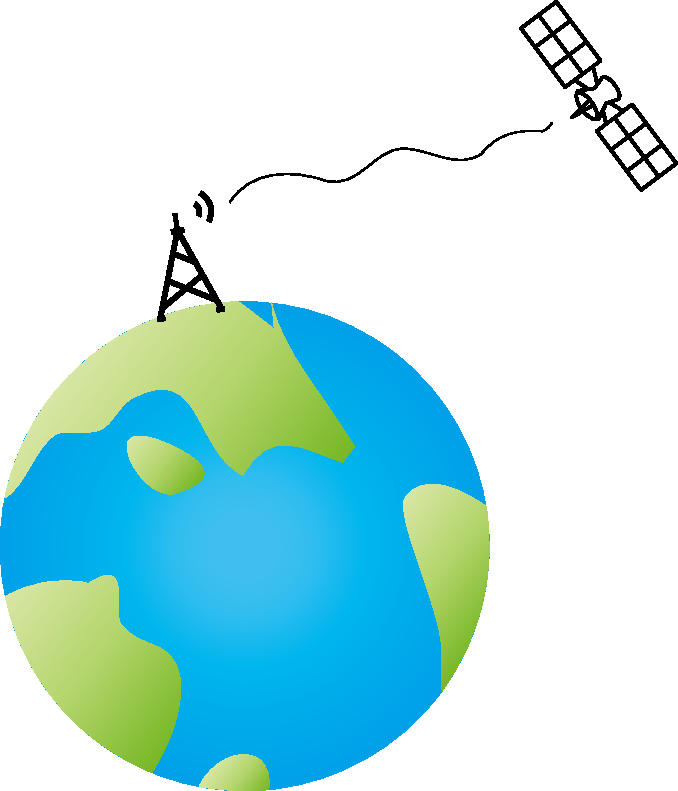
\includegraphics[width=0.3\textwidth]{images/earth-satellite.pdf}
                \label{fig:rhyolitesat}
                \end{figure}
  \item Existe um limite para a taxa de comunicação em um canal?
  \item Se o canal possuir ruido, é possível realizar uma transmissão sem erro? A qual taxa?
  \item Existe um limite superior para a quantidade de informação que podemos enviar por um canal
	dependendo das condições de ruido presente?
  \item Aumentar a taxa de transmissão acarretará num aumento da probabilidade de erro?
                \begin{figure}[h!]
                \centering
                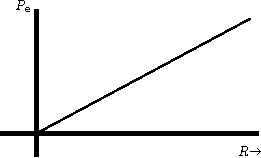
\includegraphics[width=0.3\textwidth]{images/rvspe1930.pdf}
                \label{fig:rvspe1930}
                \end{figure}
  \item Se isto ocorrer, então a única forma de ter $P_e = 0$ seria não comunicar, $R=0$.
  \end{itemize}

  \begin{example}[código de repetição]\label{ex:codrep} 
	\begin{itemize}
	\item Vamos representar um sinal por uma sequência de números.
	\item Sabemos que um sinal pode ser reconstruído perfeitamente a partir de suas amostras (teorema da amostragem, Shannon).
	\item A sequência será transmitida por um canal AM ruidoso.
	\item Possivelmente algum número será mascarado pelo ruído.
	\item Podemos repetir cada número $k$ vezes, escolhendo $k$ grande suficiente, garantindo assim que seremos capaz
	de decodificar a sequência original com probabilidade de erro pequena.
	\item A probabilidade de error diminui com $k$ e, ao mesmo tempo, a taxa de comunicação também diminui. 
	\end{itemize}

  \examplebreak
	\begin{itemize}
	\item suponha $k=3$ e a probabilidade de erro $p$
	\item mensagem a ser transmitida pelo transmissor: $s = 10110$
	\item mensagem transmitida: $t = 111 000 111 111 000$.
	\item ruído:                $n = 100 011 101 010 001$
	\item mensagem recebida: $r = t \oplus n$ (soma módulo 2)
	\item $r = 011 011 010 101 001$.
	\item decodificador: voto da maioria.
	\end{itemize}
 
  \examplebreak
	\begin{itemize}
        \item Probabilidade de inferência
	\item Regra do produto
		\begin{eqnarray}
		\Pr(s,r) &=& \Pr(s) \Pr(r|s) \nonumber \\
			&=& \Pr(r) \Pr(s|r)
		\end{eqnarray} 
	\item Regra da soma
		\begin{equation}
		\Pr(r) = \sum_s \Pr(s,r) = \Pr(s=0,r) + \Pr(s=1,r)
		\end{equation}
	\end{itemize}

  \examplebreak

        \begin{itemize}
	\item A probabilidade a posteriori de $s$ é dada
		\begin{eqnarray}
		\Pr(s|r) &=& \frac{\Pr(r|s) \Pr(s)}{\Pr(r)} \nonumber \\
			&=& \frac{\Pr(r|s) \Pr(s)}{ \Pr(r | s=0)\Pr(s=0) + \Pr(r | s=1)\Pr(s=1)}
		\end{eqnarray}
	\item $\Pr(r|s)$ : verossimilhança de $s$
	\item $P(s)$: probabilidade a priori de $s$
	\end{itemize}
 
  \examplebreak

	\begin{itemize}
	\item suponha $r=011$
		\begin{equation}
		\Pr(r | s = 0) = (1-p)\times p \times p = (1-p) p^2
		\end{equation}
		\begin{equation}
                \Pr(r | s = 1) = p \times (1-p) \times (1-p) = p(1-p)^2
                \end{equation}
	\item temos então
		\begin{equation}
		p^{\text{numero de trocas}} (1-p)^{\text{numero de concordancias entre t(s) e r}}
		\end{equation}
	\end{itemize}

  \examplebreak

        \begin{itemize}
	\item supondo $\Pr(s=0) = \Pr(s=1) = 1/2$, teremos
		\begin{equation}
		\Pr(s=1 | r =011) = \frac{ (1-p)^2 p \frac{1}{2} }{ (1-p)p^2 \frac{1}{2} + p(1-p)^2 \frac{1}{2} } = (1-p)
		\end{equation}
	\item para $p = 0.1$, por exemplo, teremos probabilidade de 90\%.
	\item $\Pr(s=1 | r) > \Pr(s=0 | r)$ então $\hat{s}=1$ é o melhor chute. 
	\end{itemize}


  \end{example}

\end{frame}


\begin{frame}[allowframebreaks]
  \frametitle{Ideia Central}
  \begin{itemize}
  \item Se escolhermos as mensagens apropriadamente, podemos ter uma situação em que teremos uma alta probabilidade
	de ter identificação univoca destas mensagens no receptor.
  \item A ideia é escolher mensagens que tendem a não criar ambiguidade no receptor.
                \begin{figure}[h!]
                \centering
                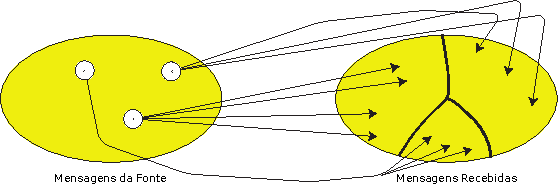
\includegraphics[width=0.5\textwidth]{images/msgsourcereceived.pdf}
		\caption{Evitar ambiguidades \citep{bilmes2013}.}
                \label{fig:msgsourcereceived}
                \end{figure}
  \item Não vamos enviar o sinal, mas sim uma representação (ou uma descrição, ou uma codificação) do sinal
	que seja adequada ao canal, de forma que o receptor seja capaz de recuperar (decodificar) o sinal.
	Adicionaremos redundância de acordo com o canal. A $P_e$ não precisa tender a zero.
  \end{itemize}

\end{frame}




\begin{frame}[allowframebreaks]
  \frametitle{Canal Discreto}

  \begin{definition}[Canal Discreto]
  Uma canal discreto é aquele em que existe um alfabeto de entrada $\mathcal{X}$, um
  alfabeto de saída $\mathcal{Y}$ e uma distribuição $p(y \mid x)$  que fornece a probabilidade
  de se observar uma saída $y$ quando a entrada é $x$.
  \end{definition}

  \begin{definition}[Canal sem memória]
  Uma canal discreto é sem memória se $y_t$, a saída no instante $t$, é independente 
  de todas entradas passadas, dado $x_t$. Isto é, $y_t \independent x_{1:t-1} \mid x_t$.
  \end{definition}

                \begin{figure}[h!]
                \centering
                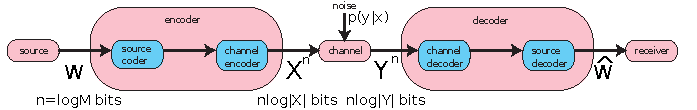
\includegraphics[width=0.9\textwidth]{images/modcom.pdf}
		\caption{Modelo de Comunicação \citep{bilmes2013}.}
                \label{fig:modcom}
                \end{figure}
  \begin{itemize}
  \item $p(x,y) = p(x)p(y|x)$ 
  \item $p(y|x)$ modela o canal sendo fixo na maioria dos casos (não temos controle sobre ele).
  \item $p(x)$ é a distribuição da fonte, que pode ser modificada (otimizada). 
  \item $p(x)$ e $p(y|x)$ são suficientes para calcularmos a informação mutua entre $X$ e $Y$.
	\begin{eqnarray}
	I(X;Y) = I_{p(x)} (X;Y) &=& \sum_{x,y} p(x) p(y|x) \log \frac{p(y|x)}{p(y)} \nonumber \\
			&=& \sum_{x,y} p(x) p(y|x) \log \frac{ p(y|x) }{ \sum_{x'} p(y|x') p(x') }
	\end{eqnarray}
  \item Para um canal fixo ($p(y|x)$ fixo), a informação mútua é uma função da distribuição $p(x)$, 
	$I(X;Y) = I_{p(x)} (X;Y)$. Esta função é concava em $p(x)$ para $p(y|x)$ dado (como visto anteriormente). 
  \item Otimizar sobre $p(x)$, para $p(y|x)$ fixo, encontrando assim a informação mútua máxima.
  \end{itemize}

  \begin{definition}[fluxo de informação]
  A taxa de fluxo de informação através de um canal é dada por $I(X;Y)$, em unidades de bits por utilização do canal.
  \end{definition}

  \framebreak

  \begin{definition}[capacidade]
  A capacidade de informação de uma canal é o máximo de fluxo de informação que podemos ter neste canal.
	\begin{equation}
	C \triangleq \max_{p(x) \in \Delta} I(X;Y)
	\end{equation}
  onde $\Delta$ é o conjunto de todas as distribuições de probabilidade sobre o alfabeto da fonte $\mathcal{X}$.
  Então $C$ é o máximo de bits que podem ser enviados através do canal por utilização do canal.
  \end{definition}

  \begin{definition}[taxa]
  A taxa $R$ de um código é medida em número de bits por utilização do canal.
  \end{definition}

\end{frame}


\subsection{Canais de Comunicação}
\begin{frame}[allowframebreaks]
  \frametitle{Canal Discreto}

  \begin{itemize}
  \item Para compressão, temos que $P_e \propto e^{-nE(R)}$. Se o expoente do erro é positivo,
	então erro $\rightarrow 0$ exponencialmente rápido à medida que o comprimento do bloco $\rightarrow \infty$.
  \item Para reduzir erro devemos ter $R > H$. Não é possível comprimir abaixo da entropia sem incorrer em erro.

                \begin{figure}[h!]
                \centering
                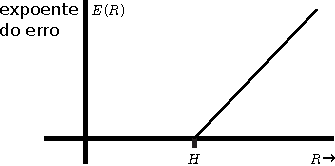
\includegraphics[width=0.3\textwidth]{images/expoenteerro.pdf}
                \label{fig:expoenteerro}
                \end{figure}

  \item Shannon mostrou que algo semelhante ocorre em comunicação. Acima de uma quantidade fundamental $C$, à medida
	que a taxa $R$ aumenta, acima de $C$, a probabilidade de erro cresce. Note que $P_e \propto e^{-nE(R)}$. 

                \begin{figure}[h!]
                \centering
                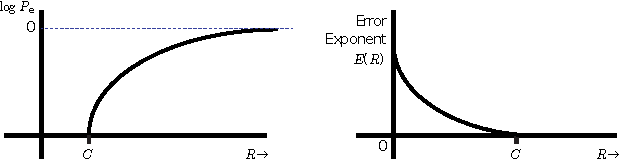
\includegraphics[width=0.8\textwidth]{images/logPe.pdf}
                \label{fig:logPe}
                \end{figure}

  \item Iremos mostrar que a única maneira de ter pouco erro é se $R < C$.
  \item Note que podemos ter comunicação sem erro se $R < C$, sendo que $C > 0$.
  \end{itemize}
\end{frame}


\begin{frame}[allowframebreaks]
  \frametitle{Exemplo: Canal Discreto Sem Memória}
  \begin{itemize}
  \item Canal binário sem ruído de $\mathcal{X} = \{0,1\}$ em $\mathcal{Y} = \{0,1\}$. 
	O diagrama mostra $p(y|x)$.

                \begin{figure}[h!]
                \centering
                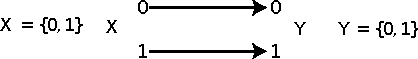
\includegraphics[width=0.5\textwidth]{images/bsc.pdf}
                \label{fig:bsc}
                \end{figure}

  \item Para este canal temos
	\begin{itemize}
	\item $p(y=0 | x = 0) = 1 = 1 - p(y=1 | x=0)$
	\item $p(y=1 | x = 1) = 1 = 1 - p(y=0 | x=1)$
	\end{itemize}
	ou seja, a saída é uma cópia da entrada.
  \item Capacidade de 1 bit. Cada vez que enviamos um bit, ele será recebido do outro lado sem erro.
  \item $I(X;Y) = H(X) - H(X|Y) = H(X)$, neste caso, teremos
	\begin{equation}
	C = \max_{p(x)} I(X;Y) = \max_{p(x)} H(X) = 1
	\end{equation}
  \item Claramente, a capacidade será alcançada se $p(0) = p(1) = 1/2$.
  \item Se $p(0)=1=1-p(1)$ teremos $I(X;Y)=0$, e assim não teremos fluxo de informação.
  \end{itemize}
\end{frame}

\begin{frame}[allowframebreaks]
  \frametitle{Exemplo: Canal com ruído e saídas sem sobreposição}
                \begin{figure}[h!]
                \centering
                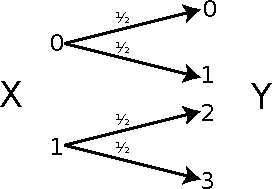
\includegraphics[width=0.4\textwidth]{images/nonc.pdf}
                \label{fig:nonc}
                \end{figure}

  \begin{itemize}
  \item Para este canal, temos
	\begin{itemize}
	\item $p(Y=0|X=0) = p(Y=1|X=0) = 1/2$
	\item $p(Y=2|X=1) = p(Y=3|X=1) = 1/2$
	\end{itemize}
  \item Se recebermos $0$ ou $1$, sabemos que $0$ foi enviado. 
	Se recebermos $2$ ou $3$, sabemos que $1$ foi enviado.
  \item $C=1$
  \item $I(X;Y) = H(X) - \underbrace{H(X|Y)}_{=0} = H(X)$.
  \item $p(0)=p(1)=1/2$ atingirá a entropia máxima.
  \end{itemize}
\end{frame}

\begin{frame}[allowframebreaks]
  \frametitle{Exemplo: Canal de permutação}
                \begin{figure}[h!]
                \centering
                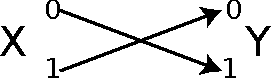
\includegraphics[width=0.3\textwidth]{images/perchan.pdf}
                \label{fig:perchan}
                \end{figure}

  \begin{itemize}
  \item Para este canal temos
	\begin{itemize}
	\item $p(Y=1|X=0) = p(Y=0|X=1) =1$
	\end{itemize}
  \item Canal de permutação.
  \item $C=1$
  \item De forma geral, para um alfabeto de tamanho $k=\vert \mathcal{X} \vert = \vert \mathcal{Y} \vert$,
	seja $\sigma$ uma permutação de forma que $Y=\sigma(X)$, então $C=\log k$.
  \end{itemize}
\end{frame}


\begin{frame}[allowframebreaks]
  \frametitle{Otimização para calcular $C$}
  \begin{itemize}
  \item Para maximizar uma função $f(x)$, é suficiente mostrar que $f(x) \leq \alpha$ para todo $x$ e 
	então encontrar $x^\ast$ tal que $f(x^\ast)=\alpha$.
  \item $x^\ast$ atinge o limite superior $\alpha$ para $f(\cdot)$.
  \item $C = \max_{p(x)} I(X;Y)$ para $p(y|x)$ fixo.
  \item A solução $p^\ast (x)$ não é necessariamente única e não será necessariamente aquela escolhida para fazer a codificação de canal.
  \item $C$ é resultado de uma otimização.
  \item $C$ é o ponto crítico para sermos capazes de codificar para o canal com probabilidade de erro tendendo a zero.
  \end{itemize}
\end{frame}


\begin{frame}[allowframebreaks]
  \frametitle{Máquina de Escrever com ruído}
                \begin{figure}[h!]
                \centering
                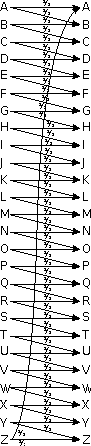
\includegraphics[width=0.06\textwidth]{images/ntype.pdf}
                \label{fig:ntype}
                \end{figure}

  \begin{itemize}
  \item 26 símbolos
  \item cada símbolo é mapeado nele mesmo ou no seu vizinho
  \item i.e. $p(A \rightarrow A) = p(A \rightarrow B) = 1/2$, etc.
  \item É possível comunicar sem erro selecionando um subconjunto que não gerará ambiguidade.
	Escolhendo A, C, E, ... ou Z, B, D, ...
  \item $A \rightarrow \{A,B\}$, $C \rightarrow \{C,D\}$, $E \rightarrow \{E,F\}$, etc.

                \begin{figure}[h!]
                \centering
                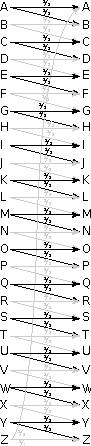
\includegraphics[width=0.06\textwidth]{images/ntype2.pdf}
                \label{fig:ntype2}
                \end{figure}
  \item $C = \log 13$ 
  \item Matematicamente
	\begin{eqnarray}
	C &=& \max_{p(x)} I(X;Y) = \max_{p(x)} \left( H(Y) - H(Y|X) \right) \nonumber \\
	&=& \max_{p(x)} H(Y) - 1 \quad \text{para $X=x$, $\exists$ duas opções} \nonumber \\
	&=& \log 26 - 1 = \log 13
	\end{eqnarray}
  \item $\max_{p(x)} H(Y) = \log 26$ pode ser alcançado quando $p(x)$ é uniforme, neste caso para qualquer $x$,
	teremos igual probabilidade de receber um dos dois $Y$s possíveis.
  \item Outra alternativa é escolher $p(x)$ de forma que a probabilidade seja nula em entradas alternadas (B, D, F, etc.).
	Neste caso, teremos também $H(Y) = \log 26$.
  \item A capacidade é a mesma em ambos casos, mas apenas um deles será utilizado para realizar uma codificação sem erro.
  \end{itemize}

\end{frame}


\begin{frame}[allowframebreaks]
  \frametitle{Canal Binário Simétrico}
                \begin{figure}[h!]
                \centering
                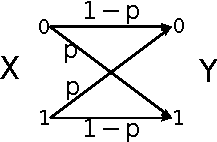
\includegraphics[width=0.3\textwidth]{images/bsch.pdf}
                \label{fig:bsch}
                \end{figure}

  \begin{itemize}
  \item Um bit enviado poderá ser alterado (\textit{flip}) com probabilidade $p$.
  \item O canal é caracterizado por
	\begin{itemize}
	\item $p(Y=1|X=0) = p = 1 -p(Y=0|X=0)$
	\item $p(Y=0|X=1) = p = 1 -p(Y=1|X=1)$
  	\end{itemize}
  \item É possível realizar comunicação sem erro com este canal?
	Sim, se a taxa de transmissão não for muito alta ($R>C$).
  \item Calcular a capacidade
	\begin{eqnarray}
	I(X;Y) &=& H(Y) - H(Y|X) \nonumber \\
		 &=&  H(Y) - \sum_x p(x) H(Y|X=x) \nonumber \\
		&=& H(Y) - \sum_x p(x) H(p) = H(Y) - H(p) \nonumber \\
		&\leq& 1 - H(p)
	\end{eqnarray}
  \item Para alcançar o limite superior, precisamos $H(Y)=1$, ou seja, $Y \sim \mathcal{U}$,
	$\Pr(Y=1) = \Pr(Y=0) = 1/2$.
  \item Temos que
	\begin{eqnarray}
	\Pr(Y=1) &=& \Pr(Y=1|X=1) \Pr(X=1) \nonumber \\
		&& + \Pr(Y=1|X=0) \Pr(X=0) \nonumber \\
		&=& (1-p) \Pr(X=1) + p (1 - \Pr(X=1)) \nonumber \\
		&=& p + (1 - 2p) \Pr(X=1) .
	\end{eqnarray}
  \item Queremos $\Pr(Y=1) = \Pr(Y=0)$, ou seja,
	\begin{eqnarray}
	\Pr(Y=0) &=& \Pr(Y=1) \nonumber \\
	1 - p - (1 - 2p) \Pr(X=1) &=& p + (1 - 2p) \Pr(X=1) \nonumber \\
	1 -2p &=& 2(1-2p) \Pr(X=1) \nonumber \\
	1 &=& 2 \Pr(X=1) \nonumber \\
	\frac{1}{2} &=& \Pr(X=1) .
        \end{eqnarray}
  \item Se $\Pr(X=1) = 1/2$ teremos $\Pr(Y=1) = p + 1/2 -p = 1/2$.
  \item Então $H(Y)=1$ se $H(X)=1$ (i.e. se $\Pr(X=1)=1/2$).
  \item $C = 1 - H(p)$ quando $X$ é uniforme.
  \item Se $p=1/2$ então $C=0$, o canal irá alterar os bits aleatoriamente com igual probabilidade, e desta forma 
	não será possível enviar informação alguma.
  \item Se $p\neq 1/2$, será possível comunicar, embora potencialmente devagar. Por exemplo,
	se $p=0.499$, então $C=2.8854 \times 10^{-6}$ bits por utilização do canal.
	Para enviar um único bit precisaremos utilizar o canal muitas vezes.
  \item Se $p=0$ ou $p=1$, teremos $C=1$ e teremos assim a maior taxa possível 
	(i.e. um bit por utilização do canal).
  \end{itemize}

\end{frame}

\subsection{Decodificação}
\begin{frame}[allowframebreaks]
  \frametitle{Decodificação}
  \begin{itemize}
  \item Podemos `decodificar' a mensagem enviada pela fonte a partir da mensagem recebida,
	da distribuição da fonte e do modelo do canal $p(y|x)$ utilizando a regra de Bayes.
	\begin{equation}
	\Pr (x|y) = \frac{\overbrace{\Pr(y|x)}^{\text{canal}} \overbrace{\Pr(x)}^{\text{fonte}} }{ \Pr(y) } = \frac{ \Pr(y|x) \Pr(x) }{ \sum_{x'} \Pr(y|x') \Pr(x')}
	\end{equation}
  \item Ao receber um determinado $y$, podemos calcular $p(x|y)$ e tomar uma decisão com base nisto.
	Ou seja, $\hat{x} = \argmax_x p(x|y)$ (decodificação de máxima verosimilhança).
  \item Ocorrerá um erro sempre que $\hat{x} \neq x$, então $\Pr(\text{erro}) = \Pr(x \neq \hat{x})$.
  \item Esta decodificação é a decodificação ótima, no sentido de minimizar o erro,
	quando $y$ é recebido para um determinado $x$ enviado,
	\begin{equation}
	\text{erro}(\overline{x}) = 1 - p(\overline{x}|y(x))
	\end{equation}
  \item Este erro será mínimo se escolhermos aquele que $\argmax_x p(x|y)$.
  \end{itemize} 
\end{frame}

\begin{frame}[allowframebreaks]
  \frametitle{Decodificação com erro mínimo}
  \begin{itemize}
  \item Computar $\Pr(x|y)$ é uma tarefa de inferência probabilística.
  \item Este problema usualmente é difícil (NP-difícil). Isto implica que
	realizar a decodificação de erro mínimo pode ter um custo exponencial (a menos que $\text{P}=\text{NP}$).
  \item Para muitos métodos de codificação, o cálculo é realizado de maneira aproximada, uma vez que não
	se conhece nenhum método rápido de calcular o erro mínimo ou realizar a decodificação de máxima verossimilhança.
  \item Métodos de inferência aproximada, por exemplo, \textit{loopy belief propagation}, \textit{message passing}, etc., 
	estes algoritmos tendem a funcionar muito bem na prática (atingem próximo de $C$).
  \end{itemize}
\end{frame}


\subsection{Canal Discreto}
%\begin{frame}[label=sldbech]
%  \frametitle{Canal Binário com Apagamento}
%                \begin{figure}[h!]
%                \centering
%                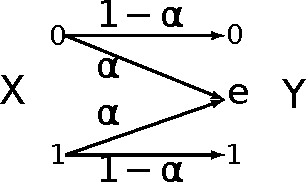
\includegraphics[width=0.3\textwidth]{images/bech.pdf}
%                \label{fig:bech}
%                \end{figure}
%\end{frame}

\begin{frame}[allowframebreaks]
  \frametitle{Canal Binário com Apagamento}
                \begin{figure}[h!]
                \centering
                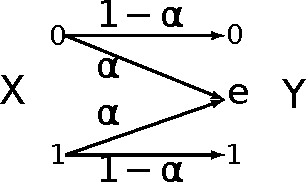
\includegraphics[width=0.3\textwidth]{images/bech.pdf}
                \label{fig:bech}
                \end{figure}

  \begin{itemize}
  \item Neste exemplo temos um símbolo que representa que o símbolo transmitido 
	foi perdido (apagado): $e$.
  \item A probabilidade disso acontecer é $\alpha$.
  \item A capacidade é calculada da seguinte forma
	\begin{eqnarray}
	C &=& \max_{p(x)} I(X;Y) = \max_{p(x)} \left( H(Y) - H(Y|X) \right) \nonumber \\
	  &=& \max_{p(x)} H(Y) - H(\alpha)
	\end{eqnarray}
  \item Temos que $H(Y) \leq \log 3$.
  \item Seja a v.a. binária $E = \{Y = e\}$, então
	\begin{equation}
	H(Y) = H(Y,E) = H(E) + H(Y|E)
	\end{equation} 
	onde utilizamos a definição de $E$ e a regra da cadeia.
  \item Seja $\pi = \Pr(X=1)$, então 
	\begin{eqnarray}
	H(Y) 	&=& H\left( \overbrace{(1-\pi)(1-\alpha)}^{\text{se }Y=0} , \overbrace{\alpha}^{\text{se }Y=e} , \overbrace{\pi(1-\alpha)}^{\text{se }Y=1} \right) \nonumber \\
		&=& H(E) + H(Y|E) \nonumber \\
		&=& H(\alpha) + (1 - \alpha) H(\pi)
	\end{eqnarray}
  \item Na ultima igualdade utilizamos $H(E) = H(\alpha)$, e 
	$H(Y|E) = \alpha H(Y|Y=e) + (1-\alpha) H(Y|Y\neq e) = \alpha \cdot 0 + (1-\alpha) H(\pi)$
                \begin{figure}[h!]
                \centering
                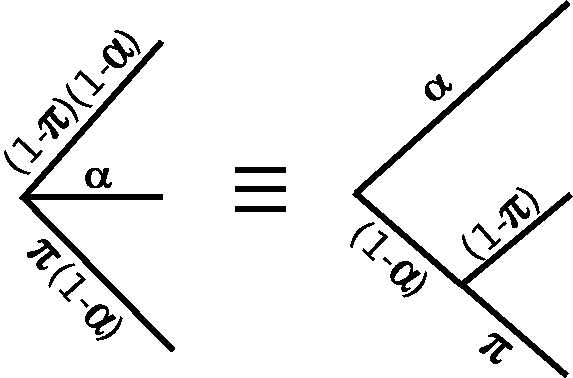
\includegraphics[width=0.4\textwidth]{images/eqvh.pdf}
                \label{fig:eqvh}
                \end{figure}

  \item Teremos então 
	\begin{eqnarray}
	C &=& \max_{p(x)} H(Y) - H(\alpha) \nonumber \\
	&=& \max_{p(x)} \left( (1-\alpha) H(\pi) + H(\alpha) \right) - H(\alpha) \nonumber \\
	&=& \max_{p(x)} (1-\alpha) H(\pi) = 1 - \alpha
	\end{eqnarray}
  \item Onde utilizamos que o máximo será obtido quando $\pi = 1/2 = \Pr(X=1) = \Pr(X=0)$.
  \item Neste canal perderemos $\alpha$\% dos bits transmitidos. A capacidade será máxima
	quando $\alpha = 0$, neste caso não haverá apagamento. 
  \end{itemize}
\end{frame}


\begin{frame}[allowframebreaks]
  \frametitle{Canal de Confusão Ternário}
                \begin{figure}[h!]
                \centering
                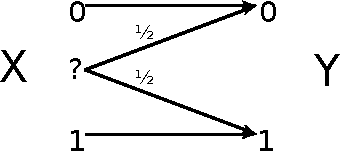
\includegraphics[width=0.3\textwidth]{images/tcc.pdf}
                \label{fig:tcc}
                \end{figure}
  \begin{itemize}
  \item $\Pr(Y=0 | X=?) = \Pr(Y=1 | X=?) = 1/2$
  \item Quando a entrada é $?$ teremos uma saída aleatória. As demais entradas são confiáveis.
  \item $C = 1$ bit.
  \item podemos obter da seguinte forma
  \begin{eqnarray}
  C &=& \max_{p(x)} I(X;Y) = \max_{p(x)} \left( H(Y) - H(Y|X) \right) \nonumber \\
    &=& \max_{p(x)} \left( H(Y) - \Pr(X = ?) \right) \nonumber \\
    &=& 1 - 0 = 1
  \end{eqnarray}
  onde utilizamos que
  \begin{eqnarray}
  H(Y|X) &=& \Pr(X=0) \underbrace{H(Y|X=0)}_{=0} + \Pr(X=?) \underbrace{H(Y|X=?)}_{=1} + \nonumber \\
	&& \Pr(X=1) \underbrace{H(Y|X=1)}_{=0} \nonumber \\
	&=& \Pr(X=?) .
  \end{eqnarray}
  \end{itemize}
\end{frame}


\subsection{Canal Simétrico}
\begin{frame}[allowframebreaks]
  \frametitle{Canal Simétrico}

  \begin{definition}
  Um canal é simétrico se as linhas da matriz de transmissão $p(y|x)$ são permutação uma das outras,
  e as colunas desta matriz também são permutação uma das outras. Um canal é fracamente simétrico
  se cada linha da matriz for uma permutação das outras linhas e todas as colunas tiverem a mesma
  soma $\sum_x p(y|x)$.
  \end{definition}

  \begin{theorem}
  Para um canal simétrico fraco, teremos
	\begin{equation}
	C = \log \vert \mathcal{Y} \vert - H(r)
	\end{equation}
  onde $r$ é a linha da matriz de transmissão. 
  \end{theorem}
  O teorema acima segue do seguinte fato
  \begin{equation}
  I(X;Y) = H(Y) - H(Y|X) = H(Y) - H(r) \leq \log \vert \mathcal{Y} \vert - H(r)
  \end{equation}

\end{frame}


\subsection{Propriedades da Capacidade de Canal}
\begin{frame}[allowframebreaks]
  \frametitle{Propriedades da Capacidade de Canal}

  \begin{itemize}
  \item $C \geq 0$, uma vez que $I(X;Y) \geq 0$,
  \item $C \leq \log \vert \mathcal{X} \vert$, uma vez que $C = \max_{p(x)} I(X;Y) \leq \max H(X) = \log \vert \mathcal{X} \vert$;
  \item de forma similar, teremos que $C \leq \log \vert \mathcal{Y} \vert$. Logo, o tamanho do alfabeto limita a capacidade de canal.
  \item $C \leq \log \left[ \min \left( \vert \mathcal{X} \vert , \vert \mathcal{Y} \vert \right) \right]$
  \item $I(X;Y) = I_{p(x)} (X;Y)$ é uma função contínua de $p(x)$, logo, existe derivada e podemos otimizá-la.
  \item $I(X;Y)$ é uma função concava de $p(x)$ para $p(y|x)$ fixo. 
	\begin{equation}
	I_{\lambda p_1 + (1-\lambda) p_2}(X;Y) \geq \lambda I_{p_1}(X;Y) + (1-\lambda) I_{p_2}(X;Y)
	\end{equation}
  \item Isto faz com que o cálculo da capacidade seja mais fácil, i.e., um máximo local é
	um máximo global, e calcular a capacidade para um modelo genérico de canal é um problema de
	otimização convexo.
  \item Temos também que $I(X;Y)$ é uma função concava de $p(y|x)$ para $p(x)$ fixo.
  \end{itemize}

\end{frame}



\subsection{Segundo Teorema de Shannon}
\begin{frame}[allowframebreaks]
  \frametitle{Segundo Teorema de Shannon}

  \begin{theorem}[Segundo Teorema de Shannon]
  $C$ é o número máximo de bits (em média, por utilização do canal) que podemos transmitir
  através de um canal de forma confiável.
  \end{theorem}

  \begin{itemize}
  \item Este teorema é um dos teoremas mais importantes do século XX.
  \item `confiável' significa: com probabilidade de erro exponencialmente decrescente à medida que
	o comprimento do bloco cresce. Podemos fazer esta probabilidade essencialmente igual a zero.
  \item Por outro lado, se tentarmos enviar mais do que $C$ bits através do canal, a probabilidade 
	de erro rapidamente vai a $1$.
  \item Problema de empacotamento de compartimentos. Temos uma região de possíveis palavras e 
	iremos empacotar tantas quantas possível, de forma a criar compartimentos sem sobreposição. 
  \item Empacotamento em compartimentos não é um particionamento, uma vez que podemos ter espaço inutilizados. 

                \begin{figure}[h!]
                \centering
                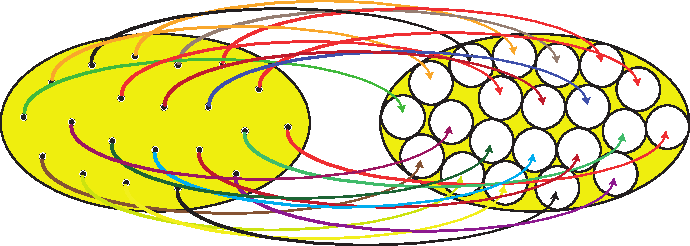
\includegraphics[width=0.5\textwidth]{images/binpack.pdf}
		\caption{Empacotamento \citep{bilmes2013}.}
                \label{fig:binpack}
                \end{figure}

  \item Ideia intuitiva: utilizar tipicidade.
  \item Existem $\approx 2^{nH(X)}$ sequências típicas, cada uma com probabilidade $2^{-nH(X)}$ e
	$p(A^{(n)}_{\epsilon}) \approx 1$, então o conjunto típico possui `toda' a probabilidade.
  \item O mesmo ocorre para a entropia condicional, ou seja, para uma entrada típica $X$,
 	existem $\approx 2^{nH(Y|X)}$ sequências de saída.
  \item Existem $2^{nH(Y)}$ sequências de saída típicas, e sabemos que $2^{nH(Y)} \geq 2^{nH(Y|X)}$.
  \item Objetivo é encontrar um subconjunto de entradas que não gerem confusão, ou seja,
	que produzam sequências na saída de forma disjunta (como ilustrado).
  \item Existem $\approx 2^{nH(Y)}$ saídas típicas (i.e., sequências em $Y$ marginalmente típicas).
  \item Existem $\approx 2^{nH(Y|X)}$ saídas possíveis dadas as entradas possíveis 
	(sequências típicas em $Y$ condicionadas em $X$), i.e., o número médio de saídas para uma
	possível entrada, que serão confundidas entre si, ou seja, na média, para um dado $X=x$ ,
	será o número aproximado de saídas correspondentes que podem existir.
  \item O número de entradas inconfundíveis será 
	\begin{equation}
	\leq \frac{2^{nH(Y)}}{2^{nH(Y|X)}} = 2^{n( H(Y) - H(Y|X) )} = 2^{nI(X;Y)}
	\end{equation}
  \item Note que em uma situação não ideal, poderia haver sobreposição das sequências
	típicas em $Y$ dado $X$, mas a melhor situação (maximizando as entradas não confundíveis) 
	é quando não há sobreposição. 

                \begin{figure}[h!]
                \centering
                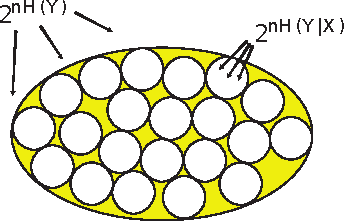
\includegraphics[width=0.3\textwidth]{images/ncset.pdf}
		\caption{Empacotamento sem sobreposição \citep{bilmes2013}.}
                \label{fig:ncset}
                \end{figure}

  \item Para maximizar o número de entradas inconfundíveis, para um canal fixo
	($p(y|x)$ fixo), devemos encontrar $p(x)$ que fornece $I(X;Y) = C$, que é
	o logaritmo do número máximo de entradas possíveis para utilização.
	$C$ é a capacidade do canal.
  \end{itemize}

\end{frame}




\subsection{Definições}
\begin{frame}[allowframebreaks]
  \frametitle{Modelos de Comunicação}
                \begin{figure}[h!]
                \centering
                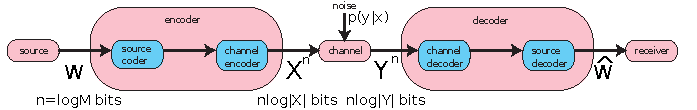
\includegraphics[width=0.8\textwidth]{images/modcom.pdf}
		\caption{Modelo de comunicação \citep{bilmes2013}.}
                \label{fig:modcomagain}
                \end{figure}
  \begin{description}
  \item[Mensagem] : $W \in \{1, \ldots, M\}$, sendo necessário $\log M$ bits por mensagem.
  \item[Sinal] $X^n(W)$ (uma palavra aleatória) será enviado através do canal.
  \item[Sinal recebido] através do canal, $Y^n \sim p(y^n|x^n)$.
  \item[Decodificação] através de um chute $\hat{W} = g(Y^n)$.
  \item[Canal discreto sem memória]: $(\mathcal{X}, p(y|x), \mathcal{Y})$.
  \item[$n$-ésima extensão do canal]: $(\mathcal{X}^n, p(y^n|x^n), \mathcal{Y}^n)$.
  \end{description}
\end{frame}

\begin{frame}[allowframebreaks]
  \frametitle{Código $(M,n)$}

  \begin{definition}[Código $(M,n)$]
  Um código $(M,n)$ para um canal $(\mathcal{X}, p(y|x), \mathcal{Y})$ é
  \begin{enumerate}
  \item um conjunto de índice $\{1,2,\ldots,M\}$;
  \item uma função de codificação $X^n : \{1,2,\ldots,M\} \rightarrow \mathcal{X}^n$ levando a palavras
	$X^n(1), X^n(2), \ldots, X^n(M)$. Cada mensagem da fonte possui uma palavra (\textit{codeword})
	e cada palavra é um código de $n$ símbolos.
  \item função de decodificação, i.e., $g: \mathcal{Y}^n \rightarrow \{1,2,\ldots,M\}$ que realiza
	um `chute' (adivinhação) sobre qual era a mensagem original dada a saída do canal.
  \end{enumerate}
  \end{definition}
  \begin{itemize}
  \item $M$ é o número de possíveis mensagens a serem enviadas, e $n$ é o número de utilizações do canal
	feitas pela palavra do código adotado.
  \item A taxa de comunicação é dada por $R = \log M / n$.
  \end{itemize}
\end{frame}

\begin{frame}[allowframebreaks]
  \frametitle{Erro}
  \begin{definition}[Probabilidade de erro $\lambda_i$ para a mensagem $i \in \{1, \ldots, M\}$]
  \begin{equation}
  \lambda_i \triangleq \Pr(g(Y^n) \neq i \mid X^n = x^n(i)) = \sum_{y^n \in \mathcal{Y}^n} p(y^n \mid x^n(i)) \mathbf{1}_{\{ g(y^n) \neq i \}}
  \end{equation}
  \end{definition}

  \begin{definition}[Probabilidade Máxima de Erro $\lambda^{(n)}$ para um código $(M,n)$]
  \begin{equation}
  \lambda^{(n)} \triangleq \max_{ i \in \{1,2, \ldots, M \}} \lambda_i
  \end{equation}
  \end{definition}

  \framebreak

  \begin{definition}[Probabilidade de Erro Média $P_e^{(n)}$]
  \begin{equation}
  P_e^{(n)} = \frac{1}{M} \sum_{i=1}^{M} \lambda_i = \Pr(I \neq g(Y^n))
  \end{equation}
  onde $I$ é uma v.a. com probabilidade $\Pr(I=i)$ de acordo com distribuição uniforme
  \begin{eqnarray}
  \Pr(I \neq g(Y^n)) = \E ( \mathbf{1}_{\{I \neq g(Y^n)\}} ) = \sum_{i=1}^M \Pr(g(Y^n) \neq i \mid X^n = x^n(i)) p(i)
  \end{eqnarray}
  onde $p(i) = 1/M$.
  \end{definition}

  \begin{itemize}
  \item O resultado central de Shannon foi mostrar que uma probabilidade de erro médio pequena
	implica em uma probabilidade máxima de erro pequena.
  \end{itemize}
\end{frame}
\note{
$P_e^{(n)}$, como definido acima, é apenas um construto matemático
da probabilidade de erro condicional $\lambda_i$, sendo ele mesmo
uma probabilidade de erro apenas se as mensagens forem escolhidas
uniformemente sob o conjunto \{1,2, \ldots, M \}.
Escolhemos uma distribuição uniforme para achar um limite no erro,
permitindo analisar o comportamento de $P_e^{(n)}$ e da probabilidade
máxima de erro $\lambda^{(n)}$, caracterizando assim o comportamento do canal
independente de como é utilizado (isto, para qualquer distribuição sobre $W$).
}


\begin{frame}[allowframebreaks]
  \frametitle{Taxa}
  \begin{definition}[Taxa $R$ de um código $(M,n)$]
  \begin{equation}
  R = \frac{\log M}{n}  
  \end{equation}
  número total de bits em uma mensagem da fonte / número total de utilizações do canal necessárias para enviar a mensagem
  \end{definition}

  \begin{definition}[Alcançabilidade de um dado canal]
  Uma taxa $R$ é alcançável para um dado canal se $\exists$ uma sequência de códigos $(\lceil 2^{nR} \rceil , n)$ tais que
  a probabilidade de erro máxima $\lambda^{(n)} \rightarrow 0$ quando $n \rightarrow \infty$.
  \end{definition}

\end{frame}


\begin{frame}[allowframebreaks]
  \frametitle{Taxa}
  \begin{definition}[Capacidade do canal discreto sem memória]
  A capacidade de uma canal discreto sem memória é a maior taxa alcançável.
  \end{definition}

  \begin{itemize}
  \item A capacidade de um canal discreto sem memória é a taxa além da qual o erro não irá mais a zero
	com o crescimento de $n$.
  \item Note que esta definição (capacidade do canal discreto sem memória) 
	é diferente da definição utilizada anteriormente ($C = \max_{p(x)} I(X;Y)$, 
	a capacidade de informação).
  \end{itemize}
\end{frame}


\subsection{Tipicidade Conjunta}
\begin{frame}[allowframebreaks]
  \frametitle{Tipicidade Conjunta}
  \begin{definition}[Tipicidade Conjunta de um conjunto de sequencias]
  Um conjunto de sequências $\{(x_{1:n} , y_{1:n})\}$ com relação a $p(x,y)$ é tipicamente
  conjunto $(\in A_{\epsilon}^{(n)})$ segundo a definição a seguir:
  \begin{eqnarray}
  A_{\epsilon}^{(n)} &=& \left\{ (x_{1:n} , y_{1:n}) \in \mathcal{X}^n \times \mathcal{Y}^n : \right. \nonumber \\ 
		&& \text{a)} \quad \vert - \frac{1}{n} \log p(x^n) - H(X) \vert < \epsilon , \quad \text{típico em x} \nonumber \\
		&& \text{b)} \quad \vert - \frac{1}{n} \log p(y^n) - H(Y) \vert < \epsilon , \quad \text{típico em y} \nonumber \\
		&& \text{c)} \quad \vert - \frac{1}{n} \log p(x^n,y^n) - H(X,Y) \vert < \epsilon , \quad \text{típico em (x,y)} \nonumber \\
		&& \left. \right\} \label{eq-tipicidade-conjunta}
  \end{eqnarray}
  com $p(x^n,y^n) = \prod_{i=1}^n p(x_i,y_i)$.
  \end{definition}

  \framebreak

                \begin{figure}[h!]
                \centering
                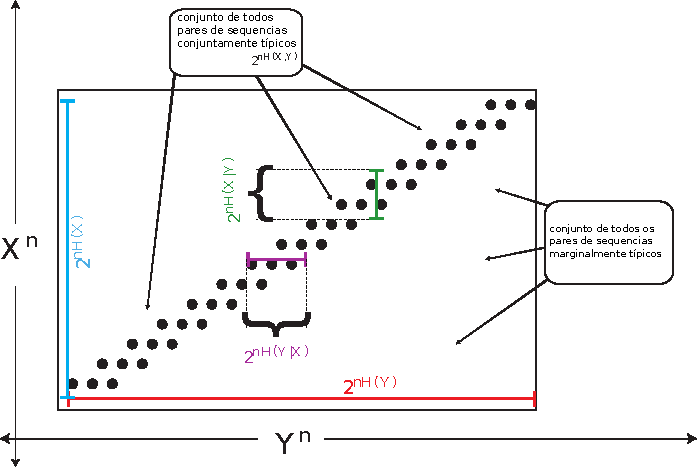
\includegraphics[width=0.5\textwidth]{images/jtyseq.pdf}
		\caption{Sequências típicas \citep{bilmes2013}.}
                \label{fig:jtyseq}
                \end{figure}

  \framebreak

  \begin{itemize}
  \item razão entre o número de sequências conjuntamente típicas e o número de sequências típicas escolhidas de forma independente 
	\begin{eqnarray}
	\frac{\text{num. seq. conj. tip.}}{\text{num. seq. tip. escolhidas ind.}} &=& \frac{2^{nH(X,Y)}}{2^{nH(X)}2^{nH(Y)}} \nonumber \\
		&=& 2^{n(H(X,Y)-H(X)-H(Y))} \nonumber \\
		&=& 2^{-nI(X;Y)}
	\end{eqnarray}
  a probabilidade de algo que seja marginalmente típico e conjuntamente típico decresce exponencialmente.
  \item Se escolhermos independentemente ao acaso duas sequências marginalmente típicas, para $X$ e $Y$, então
	a probabilidade de que teremos um sequência típica conjuntamente em $(X,Y)$ decrescerá exponencialmente com $n$,
	enquanto $I(X;Y) > 0$.
  \item Quando reduzir esta chance o máximo possível, teremos $2^{nC}$.
  \end{itemize}

  \framebreak

  \begin{theorem}[Prop. Equipartição Assintótica Conjunta]
  Seja $(X^n,Y^n) \sim p(x^n,y^n) = \prod_{i=1}^n p(x_i , y_i)$. Então
  \begin{enumerate}
  \item $\Pr \left( (X^n,Y^n) \in A_{\epsilon}^{(n)} \right) \rightarrow 1$ quando $n \rightarrow \infty$.
  \item $\vert A_{\epsilon}^{(n)} \vert \leq 2^{n(H(X,Y)+\epsilon)}$ e $(1-\epsilon) 2^{n(H(X,Y)-\epsilon)} \leq \vert A_{\epsilon}^{(n)} \vert$.
  \item Se $(\tilde{X}^n, \tilde{Y}^n) \sim p(x^n)p(y^n)$ são tirados de forma independente, então
	\begin{equation}
	\Pr \left( (\tilde{X}^n, \tilde{Y}^n) \in A_{\epsilon}^{(n)} \right) \leq 2^{-n(I(X;Y)-3\epsilon)}
	\end{equation}
	e para $n$ suficientemente grande, teremos
        \begin{equation}
        \Pr \left( (\tilde{X}^n, \tilde{Y}^n) \in A_{\epsilon}^{(n)} \right) \geq (1-\epsilon)2^{-n(I(X;Y)+3\epsilon)}
        \end{equation}
  \end{enumerate}
  \end{theorem}
  Os limites na probabilidade de sequências retiradas de forma independente serem conjuntamente típicas 
  cai exponencialmente rápido com $n$ se $I(X;Y) > 0$.

  \framebreak

  \begin{proof}[$\Pr \left( (X^n,Y^n) \in A_{\epsilon}^{(n)} \right) \rightarrow 1$]
  Pela lei fraca dos grandes números temos o seguinte
	\begin{equation}
	- \frac{1}{n} \log \Pr (X^n) \rightarrow - \E (\log p(X)) = H(X)
	\end{equation}
  então $\forall \epsilon > 0$, $\exists m_1$ tal que para $n > m_1$
	\begin{equation}
	\Pr \left( \underbrace{\vert - \frac{1}{n} \log \Pr (X^n) - H(X) \vert > \epsilon }_{=S_1}   \right) < \epsilon/3
	\end{equation}
  (apenas uma forma de reescrever o significado de convergência)
  \begin{itemize}
  \item Definimos $S_1$, o evento não típico.
  \end{itemize}

  \proofbreak

  \begin{itemize}
  \item O mesmo faremos com relação a $Y$ e $(X,Y)$.
  \item $\exists m_2$ tal que $\forall n > m_2$ teremos
        \begin{equation}
        \Pr \left( \underbrace{\vert - \frac{1}{n} \log \Pr (Y^n) - H(Y) \vert > \epsilon }_{=S_2}   \right) < \epsilon/3
        \end{equation}
  \end{itemize}

  \proofbreak

  \begin{itemize}
  \item $\exists m_3$ tal que $\forall n > m_3$ teremos
        \begin{equation}
        \Pr \left( \underbrace{\vert - \frac{1}{n} \log \Pr (X^n,Y^n) - H(X,Y) \vert > \epsilon }_{=S_3}   \right) < \epsilon/3
        \end{equation}
  \item $S_1$, $S_2$ e $S_3$ são eventos não típicos.
  \end{itemize}

  \proofbreak

  \begin{itemize}
  \item Para $n > \max(m_1, m_2, m_3)$, temos que $p(S_1 \cup S_2 \cup S_3) \leq \epsilon = 3\epsilon/3$.
  \item Não tipicidade possui probabilidade menor do que $\epsilon$, ou seja, $\Pr( A_{\epsilon}^{(n)c} ) \leq \epsilon$, 
	implicando em $\Pr( A_{\epsilon}^{(n)} ) \geq 1 - \epsilon$.
  \item A probabilidade de erro é menor do que $\epsilon$.
  \end{itemize}

  \end{proof}

  \framebreak

  \begin{proof}[$\vert A_{\epsilon}^{(n)} \vert \leq 2^{n(H(X,Y)+\epsilon)}$]
  Temos a seguinte relação
  \begin{equation}
  1 = \sum_{(x^n , y^n)} p(x^n, y^n) \geq \sum_{(x^n , y^n) \in A_{\epsilon}^{(n)}} p(x^n, y^n) \geq \vert A_{\epsilon}^{(n)} \vert 2^{-n(H(X,Y)+\epsilon)}  ,
  \end{equation} 
  logo, teremos que
  \begin{equation}
  \vert A_{\epsilon}^{(n)} \vert \leq 2^{n(H(X,Y)+\epsilon)}
  \end{equation}

  \proofbreak

  Como visto anteriormente, $\Pr(A_{\epsilon}^{(n)}) \geq 1 - \epsilon$, para $n$ grande suficiente, e assim teremos
  \begin{equation}
  1 - \epsilon \leq \sum_{(x^n , y^n) \in A_{\epsilon}^{(n)}} p(x^n, y^n) \leq \vert A_{\epsilon}^{(n)} \vert 2^{-n(H(X,Y)-\epsilon)} 
  \end{equation}
  e assim
  \begin{equation}
  \vert A_{\epsilon}^{(n)} \vert \geq (1 - \epsilon) 2^{n(H(X,Y)-\epsilon)}
  \end{equation}

  \end{proof}


  \framebreak

  \begin{proof}[Duas seq. indep. provavelmente não são conjuntamente típica]
  Seja $\tilde{X}^n$, $\tilde{Y}^n$ independente $\sim p(x^n)p(y^n)$, i.e., as duas sequências 
  são independentes entre si.

  Vamos utilizar
  \begin{equation}
  A, B \independent C  \Rightarrow A \independent C \text{ e } B \independent C
  \end{equation}
  e desta forma, teremos
  \begin{equation}
  \tilde{X}_i^n \independent \tilde{Y}_j^n , \quad \forall i,j
  \end{equation}

  \proofbreak

  Temos a seguinte derivação
  \begin{eqnarray}
  \Pr \left( (\tilde{X}^n, \tilde{Y}^n) \in A_{\epsilon}^{(n)} \right) &=& \sum_{(x^n,y^n) \in A_{\epsilon}^{(n)}} \underbrace{p(x^n)}_{\leq 2^{-n(H(X)-\epsilon)}} \underbrace{p(y^n)}_{\leq 2^{-n(H(Y)-\epsilon)}} \nonumber \\
		&\leq& \sum_{(x^n,y^n) \in A_{\epsilon}^{(n)}} 2^{-n(H(X)-\epsilon)} 2^{-n(H(Y)-\epsilon)} \nonumber \\
		&\leq& 2^{n(H(X,Y)+\epsilon)} 2^{-n(H(X)-\epsilon)} 2^{-n(H(Y)-\epsilon)} \nonumber \\
		&=& 2^{-n(I(X;Y)-3\epsilon)}
  \end{eqnarray}

  \end{proof}

\end{frame}

\subsection{Teorema da Codificação de Shannon}
\begin{frame}[allowframebreaks]
  \frametitle{Teorema da Codificação de Shannon}
  Recordando o que foi visto...
  \begin{itemize}
  \item Existem $\approx 2^{nH(X)}$ sequências típicas em $X$.
  \item Existem $\approx 2^{nH(Y)}$ sequências típicas em $Y$.
  \item O total de pares independentes é $\approx 2^{nH(X)} 2^{nH(Y)}$, mas 
	nem todos eles são conjuntamente típicos. Apenas $\approx 2^{nH(X,Y)}$ deles
	são conjuntamente típicos. 
  \item A proporção das sequências típicas independentes que são conjuntamente típicas é
	\begin{equation}
	\frac{2^{nH(X,Y)}}{2^{nH(X)} 2^{nH(Y)}} = 2^{n(H(X,Y) - H(X) - H(Y))} = 2^{-nI(X;Y)}
	\end{equation}
	e isto representa a probabilidade de que um par de sequencias marginalmente típicas, escolhido aleatoriamente, 
	seja conjuntamente típico.
  \item Se utilizarmos a tipicidade para decodificar então existem aproximadamente $2^{nI(X;Y)}$ pares de sequências
	disponíveis antes de precisarmos utilizar pares que seriam conjuntamente típicos se escolhidos aleatoriamente.
  \item Exemplo análogo: se $p(x) = 1/M$, então podemos escolher em média $M$ amostras antes de vermos um determinado $x$ em particular.
  \end{itemize}

  \framebreak

  \begin{itemize}
  \item Ideia básica é utilizar a tipicidade.
  \item Dada uma palavra recebida $y^n$, encontre um $x^n$ que seja conjuntamente típico com $y^n$.
  \item $x^n$ irá ocorrer conjuntamente com $y^n$ com probabilidade $\approx 1$, para $n$ grande suficiente. 
  \item Além disso, a probabilidade de que algum outro $\hat{x}^n$ seja conjuntamente típico com $y^n$ será
	pequena, $\approx 2^{-nI(X;Y)}$.
  \item Se utilizarmos menos que $2^{nI(X;Y)}$ palavras, então a probabilidade de que alguma outra
	sequencia seja conjuntamente típica ocorrerá com probabilidade exponencialmente decrescente, para $n$ grande suficiente. 
  \end{itemize}


  \begin{theorem}[Teorema de Codificação de Shannon]
  Todas as taxas menores do que $C \triangleq \max_{p(x)} I(X;Y)$ são alcançáveis. Especificamente,
  $\forall R < C$, existe uma sequencia de códigos $(2^{nR},n)$ com probabilidade máxima de erro 
  $\lambda^{(n)} \rightarrow 0$ quando $n \rightarrow \infty$. Por outro lado, qualquer sequencia 
  de códigos $(2^{nR},n)$ com $\lambda^{(n)} \rightarrow 0$ quando $n \rightarrow \infty$ 
  deverá ter $R < C$.
  \end{theorem}

  \begin{itemize}
  \item Enquanto não codificarmos acima da capacidade, poderemos codificar com erro nulo.
  \item Isto é verdadeiro para todo canal que possa ser representado por este modelo.
  \end{itemize}

  \framebreak

  \begin{itemize}
  \item Podemos olhar para o erro de um código em particular e encontrar os limites deste erro.
  \item Ao invés, iremos verificar a probabilidade média de erro para todos códigos gerados de forma aleatória.
  \item Iremos mostrar que este erro médio é pequeno.
  \item Isto implica que $\exists$ muitos códigos bons para que seja possível fazer a média ser pequena.
  \item Para mostrar que a probabilidade máxima de erro também é pequena, iremos descartar 50\% dos códigos.
  \item Ideia: para um dado canal $\left( \mathcal{X}, p(y|x), \mathcal{Y} \right)$ vamos tomar um código
	$(2^{nR},n)$ com taxa $R$. Isto significa que precisaremos de:
	\begin{enumerate}
	\item Conjunto de índices: $\{1, \ldots, M\}$;
	\item Codificador: $X^n: \{1, \ldots, M\} \rightarrow \mathcal{X}^n$, mapeando na palavra $X^n(i)$;
	\item Decodificador: $g: \mathcal{Y}^n \rightarrow \{1, \ldots, M\}$.
	\end{enumerate}
  \item A demonstração terá duas partes: 1) mostrar que todas as taxas $R < C$ são alcançáveis 
	(existe um código com probabilidade de erro evanescente); 2) se o erro tende a zero,
	devemos ter $R < C$. 
  \end{itemize}

  \framebreak
  
  \begin{proof}[todas as taxas $R < C$ são alcançáveis]
  \begin{itemize}
  \item Dado $R < C$, vamos assumir que utilizaremos uma distribuição $p(x)$ arbitrária e geraremos
	$2^{nR}$ palavras aleatórias utilizando a extensão $p(x^n) = \prod_{i=1}^{n} p(x_i)$.
  \item O conjunto de palavras, nosso \textit{codebook}, pode ser representado pela matriz
	\begin{equation}
	\mathcal{C} = \begin{bmatrix}
		x_1(1) & x_2(1) & x_3(1) & \ldots & x_n(1) \\
		x_1(2) & x_2(2) & x_3(2) & \ldots & x_n(2) \\
		\vdots & \vdots & \vdots & \vdots & \vdots \\
		x_1(2^{nR}) & x_2(2^{nR}) & x_3(2^{nR}) & \ldots & x_n(2^{nR}) 
		\end{bmatrix}
	\end{equation}
	Desta forma, existe $2^{nR}$ palavras (\textit{codewords}), de comprimento $n$, 
	geradas por $p(x)$, cada uma em uma linha da matriz.
  \end{itemize}

  \proofbreak

  \begin{itemize}
  \item O \textit{codebook} $\mathcal{C}$ é aleatório e terá probabilidade $\Pr(\mathcal{C})$.
  \item Para enviar qualquer mensagem $w \in \{1, \ldots, M=2^{nR}\}$, devemos enviar a palavra
	correspondente $x_{1:n}(w)=\left( x_1(w), x_2(w), \ldots, x_n(w) \right)$.
  \item Podemos calcular a probabilidade de uma dada palavra $w \in \{1, \ldots, M\}$ da seguinte forma
	\begin{equation}
	p\left( x^n(w) \right) = \prod_{i=1}^{n} p\left( x_i(w) \right) , \quad w \in \{1, \ldots, M\} .
	\end{equation}
  \end{itemize}

  \proofbreak

  \begin{itemize}
  \item A probabilidade de todo o \textit{codebook} será dada por
	\begin{equation}
	p(\mathcal{C}) = \prod_{w=1}^{2^{nR}} \prod_{i=1}^n p\left( x_i(w) \right) .
	\end{equation}
  \end{itemize}

  \proofbreak

  Considere o seguinte esquema de codificação/decodificação:
	\begin{enumerate}
	\item Gere um \textit{codebook} aleatório, como descrito anteriormente, de acordo 
		com uma distribuição $p(x)$;
	\item O \textit{codebook} é conhecido pelo transmissor/receptor (também conhecem $p(y|x)$). 
	\item Vamos gerar mensagens $W$ de acordo com uma distribuição uniforme, ou seja,
		todas mensagens serão equiprováveis, $p(W=w) = 2^{-nR}$ para $w=1, \ldots, 2^{nR}$.
	\item Escolhemos uma mensagem $w$ e enviamos a palavra correspondente $x^n(w)$ através do canal.
	\asuivre
	\end{enumerate}
	\proofbreak
	\begin{enumerate}
	\suite
	\item A mensagem recebida $Y^n$ será dada de acordo com a seguinte distribuição
		\begin{equation}
		Y^n \sim p(y^n \mid x^n(w)) = \prod_{i=1}^{n} p(y_i | x_i(w))
		\end{equation}
	\item O sinal é decodificado utilizando a decodificação através do conjunto típico (será descrito adiante).	
	\end{enumerate}
 
  \proofbreak

  Decodificador utilizando conjunto típico.
  Vamos decodificar $\hat{w}$ se
	\begin{enumerate}
	\item $\left( x^n(\hat{w}), y^n \right)$ é conjuntamente tipico, ou seja, $\left( x^n(\hat{w}), y^n \right) \in A_{\epsilon}^{(n)}$;
	\item $\hat{w}$ é único, ou seja, $\nexists w'$ tal que $\left( x^n(w'), y^n \right) \in A_{\epsilon}^{(n)}$ para $w' \neq \hat{w}$.
	\end{enumerate}
  Se estas duas condições não acontecerem, teremos um erro e a saída será um inteiro especial `0' (para designar erro).
  Três tipos de erro podem ocorrer:
  \begin{enumerate}[a)]
  \item  $\exists w' \neq \hat{w}$ tal que $\left( x^n(w'), y^n \right) \in A_{\epsilon}^{(n)}$, i.e., 
	existe mais do que uma mensagem típica;
  \item $\nexists \hat{w}$ tal que $\left( x^n(\hat{w}), y^n \right)$ é conjuntamente tipico;
  \item se $\hat{w} \neq w$, i.e., a palavra errada é conjuntamente típica.
  \end{enumerate}

  \proofbreak
  obs.: decodificação de máxima verossimilhança é ótima, já a decodificação pelo conjunto típico não é ótima,
	entretanto será suficiente para mostrar o resultado pretendido. 

  \proofbreak
  
  Vejamos três medidas de qualidade que poderemos utilizar.
  \begin{enumerate}
  \item Erro específico do código:
	\begin{equation}
	P_e^{(n)} (\mathcal{C}) = \Pr(\hat{w} \neq w \mid \mathcal{C}) = \frac{1}{2^{nR}} \sum_{i=1}^{2^{nR}} \lambda_i
	\end{equation}
	onde (conforme definido anteriormente)
	\begin{equation}
	\lambda_i \triangleq \Pr(g(Y^n)) \neq i \mid X^n = X^n(i)) = \sum_{y^n \in \mathcal{Y}^n} p(y^n \mid X^n(i)) \mathbf{1}_{\{ g(y^n) \neq i \}} .
	\end{equation}
	Note que $\mathcal{C}$ é uma v.a..
  \asuivre
  \end{enumerate}
 
  \proofbreak
  
  \begin{enumerate}
  \suite
  \item Erro médio entre todos códigos gerados aleatoriamente 
	(vamos tomar o valor esperado do erro específico de um código)
	\begin{eqnarray}
	\Pr(\varepsilon) &=& \E[P_e^n(\mathcal{C})] \nonumber \\
		&=& \sum_{\mathcal{C}} \Pr(\mathcal{C}) \Pr(\hat{W} \neq W | \mathcal{C}) \nonumber \\
		&=& \sum_{\mathcal{C}} \Pr(\mathcal{C}) P_e^{(n)}(\mathcal{C})
	\end{eqnarray}
	Isto será mais fácil de analisar do que $P_e$.
  \asuivre
  \end{enumerate}

  \proofbreak

  \begin{enumerate}
  \suite
  \item Erro máximo de um código:
	\begin{equation}
	P_{\mathcal{C}, \max} (\mathcal{C}) = \max_{i \in \{1,2, \ldots, M\}} \lambda_i .
	\end{equation}
	Queremos mostrar que se $R<C$, então existe um \textit{codebook} $\mathcal{C}$ tal que
	$P_{\mathcal{C}, \max} \rightarrow 0$ (e se $R > C$, então $P_{\mathcal{C}, \max} \rightarrow 1$).
  \end{enumerate}

  \proofbreak

  Procedimento:
  \begin{enumerate}
  \item Expandir o erro médio e mostrar que ele é pequeno;
  \item Deduzir que $\exists$ ao menos 1 código com erro pequeno;
  \item Mostrar que isto pode ser modificado para termos uma probabilidade de erro máximo pequena.
  \end{enumerate}

  \proofbreak
  Erro médio
  \begin{eqnarray}
  \Pr(\varepsilon) &=& \sum_{\mathcal{C}} \Pr(\mathcal{C}) P_e^{(n)}(\mathcal{C}) = \sum_{\mathcal{C}} \Pr(\mathcal{C}) \frac{1}{2^{nR}} \sum_{w=1}^{2^{nR}} \lambda_w(\mathcal{C}) \nonumber \\
	&& \text{\small valor médio, entre os codebooks, dos } \nonumber \\
	&& \text{\small valores médios entre as palavras em um coodebook} \nonumber \\
	&=& \frac{1}{2^{nR}} \sum_{w=1}^{2^{nR}} \sum_{\mathcal{C}} \Pr(\mathcal{C}) \lambda_w(\mathcal{C}) 
  \end{eqnarray}

  \proofbreak

  mas
  \vspace{-0.75cm}
  \begin{eqnarray}
  \sum_{\mathcal{C}} \Pr(\mathcal{C}) \lambda_w(\mathcal{C}) &=& \nonumber \\
  \sum_{\mathcal{C}} \overbrace{\Pr\left( g(Y^n) \neq w \mid X^n = x^n(w) \right)}^{\lambda_w(\mathcal{C})} \overbrace{\Pr\left( x^n(1), \ldots, x^n(2^{nR}) \right)}^{\Pr(\mathcal{C})} &=& \nonumber \\
  \sum_{\mathcal{C}} \underbrace{ \Pr\left( g(Y^n) \neq w \mid X^n = x^n(w) \right) \overbrace{\Pr\left( x^n(1), \ldots, x^n(2^{nR}) \right)}^{ \prod_{i=1}^{2^{nR}} \Pr(x^n(i)) }  }_{\text{coisa}} &=& \nonumber \\
  \sum_{ x^n(1), \ldots, x^n(2^{nR}) } \text{coisa} 
  \end{eqnarray}

  \proofbreak

  \vspace{-0.5cm}
  \begin{eqnarray}
  \sum_{\mathcal{C}} \Pr(\mathcal{C}) \lambda_w(\mathcal{C}) &=& \sum_{ x^n(1), \ldots, x^n(2^{nR}) } \text{coisa} \nonumber \\
	&& \text{somatório com } \underbrace{2^n \cdots 2^n}_{2^{nR} \text{vezes}} = 2^{n2^{nR}} \text{termos} \nonumber \\
  	&=& 
  \sum_{ \substack{ x^n(1), \ldots, x^n(w-1),  \\ x^n(w+1), \ldots, x^n(2^{nR}) } } \sum_{x^n (w)} \text{coisa} 
  \end{eqnarray}

  \proofbreak

  Temos também que
  \begin{eqnarray}
  \text{coisa} &=& \prod_{i=1}^{2^{nR}} \Pr(x^n(i)) \lambda_w(\mathcal{C}) \nonumber \\
  	&=& \left( \prod_{ \substack{ i=1 \\ i \neq w} }^{2^{nR}} \Pr(x^n(i)) \right) \underbrace{ \Pr(x^n(w)) \lambda_w(\mathcal{C}) }_{\text{termo em }w}
  \end{eqnarray}
 
  \proofbreak
 
  \vspace{-0.5cm} 
  \begin{eqnarray}
  & & \\
  \sum_{\mathcal{C}} \Pr(\mathcal{C}) \lambda_w(\mathcal{C}) &=&  \nonumber \\
  \underbrace{ \sum_{ \substack{ x^n(1), \ldots, x^n(w-1),  \\ x^n(w+1), \ldots, x^n(2^{nR}) } } \underbrace{p\left( \substack{ x^n(1), \ldots, x^n(w-1), \\ x^n(w+1), \ldots, x^n(2^{nR}) } \right)}_{\prod_{i \neq w} \Pr(x^n(i)) } }_{=1}  \sum_{x^n (w)} \Pr\left( g(Y^n) \neq w \mid X^n = x^n(w) \right)  \Pr\left( x^n(w) \right)  &=&  \nonumber
  \end{eqnarray}
  O primeiro termo é igual à $1$ pois corresponde à soma dos termos de uma distribuição conjunta ($2^{nR}-1$ termos).

  \proofbreak
  \vspace{-0.5cm}
  \begin{eqnarray}
  \sum_{\mathcal{C}} \Pr(\mathcal{C}) \lambda_w(\mathcal{C}) &=& \nonumber \\
  \sum_{x^n (w)} \Pr\left( g(Y^n) \neq w \mid X^n = x^n(w) \right) \Pr\left( x^n(w) \right) &=& \nonumber \\
  \sum_{x^n \in \mathcal{X}^n} \Pr\left( g(Y^n) \neq 1 \mid X^n = x^n(1) \right) \Pr\left( x^n(1) \right)
  \end{eqnarray}

  \proofbreak
  
  Na equação anterior utilizamos que o resultado é o mesmo para qualquer $w$, logo, sem perca
  de generalidade, escolhemos $w=1$, uma mensagem qualquer. Teremos assim
  \begin{equation}
  \sum_{\mathcal{C}} \Pr(\mathcal{C}) \lambda_w(\mathcal{C}) = \sum_{\mathcal{C}} \Pr(\mathcal{C}) \lambda_1(\mathcal{C}) = \beta
  \end{equation}

  \proofbreak

  Exemplo: intuição sobre como chegamos a $\beta$. 

                \begin{figure}[h!]
                \centering
                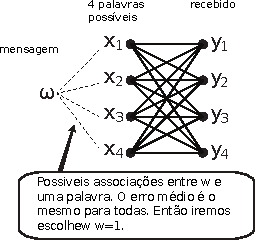
\includegraphics[width=0.3\textwidth]{images/wxyass.pdf}
                \label{fig:wxyass}
                \end{figure}

  \proofbreak
  
  O erro então é igual a: prob. de escolher $x_1$ para $w$ e não escolher $y_1$ + 
			prob. de escolher $x_2$ para $w$ e não escolher $y_2$ + $\ldots$
 
  Teremos o mesmo resultado para todo $w \in \{1,2,\ldots,M\}$, então podemos selecionar $w=1$.

  Obtemos assim
  \begin{equation}
  \Pr(\varepsilon) = \sum_{\mathcal{C}} \Pr(\mathcal{C}) P_e^{(n)}(\mathcal{C}) =  \frac{1}{2^{nR}} \sum_{w=1}^{2^{nR}} \beta = \sum_{\mathcal{C}} \Pr(\mathcal{C}) \lambda_1(\mathcal{C}) = \beta
  \end{equation}
   onde $\beta = \Pr(\varepsilon \mid W=1)$.

  \proofbreak

  Vamos definir eventos de erro aleatórios (considerando $w=1$)
  \begin{equation}
  E_i \triangleq \left\{ (x^n(i),y^n) \in A_{\epsilon}^{(n)} \right\} \text{ para } i=1,\ldots,2^{nR}
  \end{equation}
  Assumindo que a entrada é $x^n(1)$, então não haver erro é equivalente a
  \begin{equation}
  E_1 \cap \neg (E_2 \cup E_3 \cup \ldots \cup E_M).
  \end{equation}
 
  \proofbreak

  Tipos de erro:
  \begin{itemize}
  \item $E_1^c$ significa que a palavra transmitida e recebida não são conjuntamente típicas (erro tipo B).
  \item $E_2 \cup E_3 \cup \ldots \cup E_{2^{nR}}$ é uma das seguintes possibilidades:
	\begin{itemize}
	\item erro tipo C: a palavra errada é conjuntamente típica com a sequência recebida;
	\item erro tipo A: mais do que 1 palavra é conjuntamente típica com a sequência recebida.
	\end{itemize}
  \end{itemize}

  \proofbreak

                \begin{figure}[h!]
                \centering
                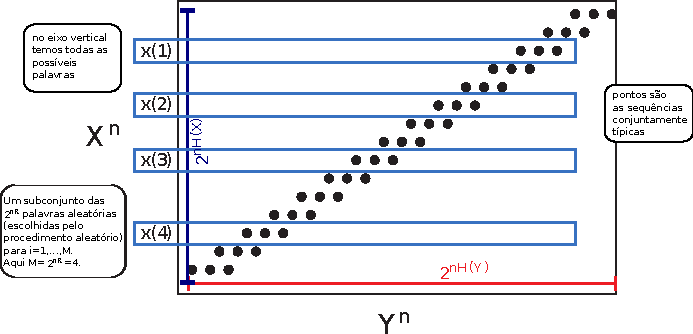
\includegraphics[width=0.6\textwidth]{images/mesmap.pdf}
                \label{fig:mesmap}
                \end{figure}

  \proofbreak
		\vspace{-0.25cm}
                \begin{figure}[h!]
                \centering
                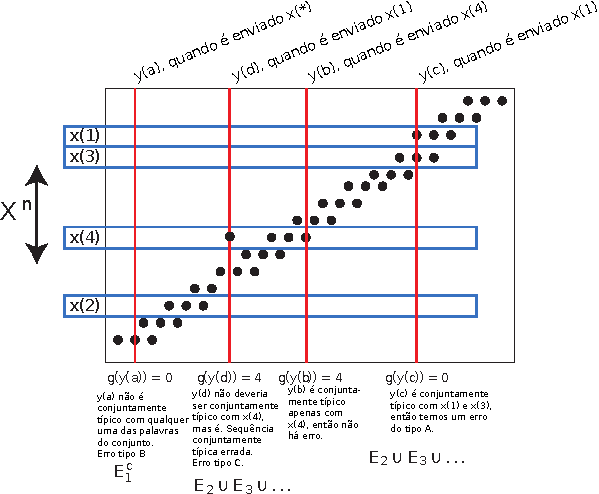
\includegraphics[width=0.4\textwidth]{images/codmap.pdf}
                \label{fig:codmap}
                \end{figure}
  \proofbreak
 
  Objetivo: limitar a probabilidade de erro.  
  \begin{eqnarray}
  \Pr(\varepsilon \mid W = 1) &=& \Pr(E_1^c \cup E_2 \cup E_3 \ldots) \nonumber \\
			&\leq& \Pr(E_1^c) + \sum_{i=2}^{2^{nR}} \Pr(E_i) 
  \end{eqnarray}
  Assim teremos
  \begin{equation}
  \Pr(E_1^c) = \Pr(A_{\epsilon}^{(n)c}) \rightarrow 0  \quad \text{quando } n \rightarrow \infty
  \end{equation}
  então $\forall \epsilon$, $\exists n_0$ tal que
  \begin{equation}
  \Pr(E_1^c) \leq \epsilon , \quad \forall n > n_0
  \end{equation}

  \proofbreak

  Ainda, como temos um processo de geração de código aleatório, as sequências $X^n$ geradas 
  para diferentes mensagens são independentes (sem perca de generalidade podemos selecionar $w=1$)
  \begin{equation}
  X^n(1) \independent X^n(i) \Rightarrow Y^n \independent X^n(i) , \text{ para } i \neq 1
  \end{equation}
  Teremos então que, para $i \neq 1$,
  \begin{equation}
  \Pr ( \underbrace{(X^n(i) , Y^n)}_{\text{eventos indep.}} \in A_{\epsilon}^{(n)} ) \leq 2^{-n (I(X;Y) - 3 \epsilon)} ,
  \end{equation}
  pela Prop. da Eq. Ass. conjunta.
 
  Isto nos permitirá limitar o erro, enquanto $I(X;Y) > 3\epsilon$.

  \proofbreak

  Teremos assim

  \vspace{-0.75cm}
  \begin{eqnarray}
  \Pr(\varepsilon) &\leq& \Pr(E_1^c) + \sum_{i=2}^{2^{nR}} \Pr(E_i) \nonumber \\
	&\leq& \epsilon + \sum_{i=2}^{2^{nR}} 2^{-n(I(X;Y)-3\epsilon)} \nonumber \\
	&=& \epsilon + (2^{nR} - 1) 2^{-n(I(X;Y)-3\epsilon)} \nonumber \\
	&\leq& \epsilon + 2^{3n\epsilon} 2^{-n(I(X;Y)-R)} \nonumber \\
	&=& \epsilon + 2^{-n((I(X;Y)-3\epsilon)-R)} \\
	&\leq& 2 \epsilon \text{, quando $n$ for grande suficiente}
  \end{eqnarray}
  \vspace{-0.3cm}
  Isto é verdadeiro enquanto $I(X;Y) -3\epsilon > R$.

  \proofbreak

  \begin{itemize}
  \item Se escolhermos $R < I(X;Y)$ (estritamente), podemos encontrar $\epsilon$ e $n$ tais que
	a probabilidade média de erro $\Pr(\varepsilon) < 2\epsilon$, possa ser feita tão pequena
	quão desejado.
  \item Precisamos encontrar a probabilidade máxima de erro, a partir da probabilidade média, e então avaliar o limite.
  \item Vamos escolher $p^\ast(x) = \argmax_{p(x)} I(X;Y)$ ao invés de $p(x)$ uniforme, para assim mudar
	a condição $R < I(X;Y)$ para $R < C$. Isto nos fornecerá um limite maior.
  \end{itemize}
  \proofbreak
  \begin{itemize}
  \item Se $\Pr(\varepsilon) \leq 2 \epsilon$, então deve existir um código específico $C^\ast$ tal que
	\begin{equation}
	P_e^{(n)} (C^\ast) \leq 2 \epsilon
	\end{equation}
	(se a média é menor ou igual a $2\epsilon$, então devemos ter ao menos um valor menor ou igual a $2\epsilon$).
  \end{itemize}

  \proofbreak

  \begin{eqnarray}
  P_e^{(n)} (C^\ast) &=& \frac{1}{2^{nR}} \sum_{i=1}^{2^{nR}} \lambda_i (C^\ast) \nonumber \\
	&=& \frac{1}{2^{nR}} \sum_{i: \lambda_i < 4\epsilon} \lambda_i (C^\ast) + \frac{1}{2^{nR}} \sum_{i: \lambda_i \geq 4\epsilon} \lambda_i (C^\ast) \nonumber \\
	&\leq& 2 \epsilon
  \end{eqnarray}

  \proofbreak

  Suponha que mais da metade dos índices possuam erro $\geq 4 \epsilon$ 
  (i.e., $\vert \{i: \lambda_i \geq 4 \epsilon \} \vert > 2^{nR}/2$ ). Assim, teremos
  \begin{equation}
  \frac{1}{2^{nR}} \sum_{i: \lambda_i \geq 4\epsilon} \lambda_i \geq \frac{1}{2^{nR}} \sum_{i: \lambda_i \geq 4\epsilon} 4 \epsilon = \frac{1}{2^{nR}} \vert \{i: \lambda_i \geq 4 \epsilon \} \vert 4 \epsilon > \frac{1}{2} 4 \epsilon = 2\epsilon
  \end{equation}
  Isto não é possível, pois a probabilidade de erro é $\leq 2\epsilon$ e uma parte dos termos que a compõem não pode ser $> 2\epsilon$.
  Desta forma, no máximo metade das palavras possuem erro $\geq 4\epsilon$.

  \proofbreak

  \begin{itemize}
  \item Como no máximo metade das palavras possuem erro $\geq 4\epsilon$, teremos
  \begin{equation}
  \vert \{i: \lambda_i \geq 4 \epsilon \} \vert \leq \frac{2^{nR}}{2} \Rightarrow \vert \{i: \lambda_i < 4 \epsilon \} \vert \geq \frac{2^{nR}}{2}
  \end{equation}
  \item Vamos criar um novo \textit{codebook} eliminando todas as palavras ruins 
	(i.e., aquelas com índice $\{i: \lambda_i \geq 4 \epsilon\})$. Eliminamos assim
	no máximo metade das palavras.
  \item O tamanho do conjunto de palavras remanescentes é $\geq 2^{nR}/2 = 2^{nR-1} = 2^{n(R-1/n)}$ 
	(ao menos metade das palavras iniciais). Todas elas possuem probabilidade de erro máxima $\leq 4\epsilon$.
  \end{itemize}

  \proofbreak
  \begin{itemize}
  \item Iremos agora codificar com taxa $R' = R-1/n \rightarrow R$ quando $n \rightarrow \infty$, mas
	para esta nova sequência de códigos, a probabilidade máxima de erro $\lambda^{(n)} \leq 4\epsilon$,
	que pode ser feita tão pequena quanto desejável.
  \end{itemize}
  \end{proof}

  \begin{itemize}
  \item Utilizamos uma codificação aleatória para provar que se $R<C$, então existe uma sequência de códigos $(2^{nR},n)$ 
  com probabilidade de erro máxima $\lambda^{(n)} \rightarrow 0$ quando $n \rightarrow \infty$.

  \item Este código pode não ser o melhor código, mas é suficiente. Temos a prova de que existe tal código.
 
  \item Existem muitos código bons, como por exemplo, código turbo e código de Gallager 
	(ou verificação de paridade de baixa densidade).
  \end{itemize}


  \framebreak

  \begin{proof}[proposição inversa]
  \begin{itemize}
  \item Queremos mostrar que qualquer sequência de códigos $(2^{nR},n)$ com $\lambda^{(n)} \rightarrow 0$ deve ter $R \leq C$.
  \item Inicialmente, vamos considerar o caso em que $P_e^{(n)} = 0$, pois tal caso é mais simples.
  \end{itemize}

  \proofbreak

  \begin{itemize}
  \item Se $P_e^{(n)} = 0$, então $H(W \mid Y^n) = 0$ (não há incerteza).
  \item Para simplificar, vamos assumir que a mensagem tem distribuição uniforme em $\{1, 2, \ldots, M\}$.
	Desta forma, $H(W) = nR = \log M$. Esta suposição será suficiente, pois esta é a taxa máxima quando temos $M$ mensagens.
	\begin{eqnarray}
	nR &=& H(W) = \underbrace{H(W \mid Y^n)}_{=0} + I(W;Y^n) = I(W;Y^n) \nonumber \\
		&\leq& I(X^n;Y^n)
	\end{eqnarray}
	pois $W \rightarrow X^n \rightarrow Y^n$ é uma cadeia de Markov e podemos aplicar a desigualdade de processamento de dados.
  \end{itemize}
  
  \proofbreak

	\vspace{-0.75cm}
       \begin{eqnarray} 
	nR &\leq& I(X^n;Y^n) \nonumber \\
		&=& H(Y^n) - H(Y^n \mid X^n) \nonumber \\
		&& \text{utilizando a regra da cadeia} \nonumber \\
		&=& H(Y^n) - \sum_{i=1}^{n} H(Y_i \mid Y_{1:i-1}, X^n) 
	\end{eqnarray}

  \proofbreak

	\begin{eqnarray} 
        nR &\leq& H(Y^n) - \sum_{i=1}^{n} H(Y_i \mid Y_{1:i-1}, X^n) \nonumber \\
		&& \text{mas $Y_i \independent \{ Y_{1:i-1}, X_{1:i-1}, X_{i+1:n} \} \mid X_i$ ,} \nonumber \\
		&& \text{pela definição de canal discreto sem memória} \nonumber \\
		&=& H(Y^n)  - \sum_{i=1}^{n} H(Y_i \mid X_i) \leq \sum_{i} \left( H(Y_i) - H(Y_i \mid X_i) \right) \nonumber \\
		&=& \sum_{i=1}^{n} I(Y_i;X_i) \leq nC
	 \end{eqnarray}

  \proofbreak

  \begin{itemize}
  \item Mostramos que $R \leq C$ quando $P_e^{(n)} = 0$.
  \item Mostramos ainda que $H(W) \leq nC$, isto significa que $\max_p H_p(W) \leq nC$,
	\begin{equation}
	H(W) \leq \max_p H_p(W) = nR \leq nC
	\end{equation}
	e $R \leq C$ independente da distribuição da fonte.
  \end{itemize}
  \end{proof}

  
  \framebreak
  \begin{itemize}
  \item O seguinte Lemma também foi mostrado
	\begin{lemma}
	\begin{equation}
	I(X^n \mid Y^n) \leq nC
	\end{equation}
	\end{lemma}
  \item Na continuação, iremos utilizar a desigualdade de Fano:
	\begin{equation}
	H(X \mid Y) \leq 1 + P_e \log \vert \mathcal{X} \vert
	\end{equation}
  \end{itemize}
 
  \framebreak
 
  \begin{theorem}[Fano]
  Para um canal discreto sem memória com \textit{codebook} $\mathcal{C}$ e mensagens de entrada 
  uniformemente distribuídas $(H(W) = nR)$ e $P_e{(n)} = \Pr(W \neq g(Y^n))$, então
	\begin{equation}
	H(X^n \mid Y^n) \leq 1 + P_e{(n)} nR
	\end{equation}
  \end{theorem}
  \framebreak 
  \begin{proof}
  Seja $E \triangleq \mathbf{1}_{\{ W \neq \hat{W} \}}$, então
	\begin{eqnarray}
	H(E, W \mid Y^n) &=& H(W \mid Y^n) + \underbrace{H(E \mid Y^n , W)}_{=0} \nonumber \\
			&=& \underbrace{H(E \mid Y^n)}_{\leq 1} + H(W \mid Y^n , E)
	\end{eqnarray}
  \proofbreak
  Vamos utilizar que 
	\begin{eqnarray}
	H(W \mid Y^n , E) &=& \underbrace{\Pr(E=0)}_{1 - P_e^{(n)}} \underbrace{H(W \mid Y^n, E=0)}_{=0} \nonumber \\
			&& + \underbrace{\Pr(E=1)}_{P_e^{(n)}} \underbrace{H(W \mid Y^n, E=1)}_{\leq\log(2^{nR}-1)} \nonumber \\
			&& \text{\small se houve erro, então sobraram $2^{nR}-1$ opções} \nonumber \\
			&\leq& P_e^{(n)} nR
        \end{eqnarray}
  \proofbreak
  Teremos assim 
	\begin{equation}
	H(W \mid Y^n) \leq 1 + P_e^{(n)} nR
	\end{equation}
  e, utilizando $X^n = X^n(W)$, funções de uma v.a. só podem reduzir a entropia, teremos 
  a desigualdade de Fano
	\begin{equation}
	H(X^n \mid Y^n) \leq H(W \mid Y^n) \leq 1 + P_e^{(n)} nR
        \end{equation}

  \end{proof}
 
  \framebreak

  Continuando a demonstração da proposição inversa...
  Ou seja, qualquer sequência de códigos $(2^{nR},n)$ com $\lambda^{(n)} \rightarrow 0$ deve ser tal que $R \leq C$
  \begin{proof}[$\lambda^{(n)} \rightarrow 0$ quando $n \rightarrow 0$ $\Rightarrow$ $R < C$]
  \begin{itemize}
  \item A probabilidade média vai para zero se a probabilidade máxima for:
	$\lambda^{(n)} \rightarrow 0 \Rightarrow P_{e}^{(n)} \rightarrow 0$, onde $P_{e}^{(n)} = \frac{1}{2^{nR}} \sum_{i=1}^{2^{nR}} \lambda_i$.
  \item Outra vez, para facilitar, vamos fazer $H(W) = nR$ (i.e., $W$ com distribuição uniforme sobre $\{1,2,\ldots, M=2^{nR}\}$)
	(isto não afeta a relação entre $R$ e $C$).
  \item Então, $\Pr(W \neq \hat{W}) = P_e^{(n)} = \frac{1}{M} \sum_{i=1}^M \lambda_i$, como visto anteriormente.
  \end{itemize}

  \proofbreak

  \begin{eqnarray}
  nR &=& H(W) = H(W \mid Y^n) + I(W; Y^n) \\
	&\leq& H(W \mid Y^n) + I(X^n(W);Y^n) \quad \text{\small pois } W \rightarrow X^n \rightarrow Y^n \nonumber \\
	&\leq& 1 + P_e^{(n)} nR + I(X^n(W);Y^n)	\quad \text{\small Fano} \nonumber \\
	&\leq& 1 + P_e^{(n)} nR + nC \quad \text{\small lemma anterior} 
  \end{eqnarray}
  Logo teremos que $R \leq P_e^{(n)} R + 1/n +C$.

  Fazendo $n \rightarrow \infty$, $P_e^{(n)} \rightarrow 0$ e $1/n \rightarrow 0$, teremos 
	\begin{equation}
	R < C
	\end{equation}
  \end{proof}

  \framebreak
  
  Rearranjando os termos da equação anterior, podemos escrever
  \begin{equation}
   P_e^{(n)} \geq 1 - \frac{C}{R} - \frac{1}{nR} .
  \end{equation}
  Isto significa que:
  \begin{itemize}
  \item se $n \rightarrow \infty$ e $R>C$, então o limite inferior do erro é estritamente positivo e depende de $1 - C/R$.
  \item Mesmo para $n$ pequeno, $P_e^{(n)} > 0$, pois caso contrário, se $P_e^{(n)} = 0$ para algum código,
	poderemos concatenar o código e criar um código maior com a mesma taxa, contradizendo $P_e^{(n)} > 0$.
  \end{itemize}

  \framebreak

  O limite inferior da probabilidade de erro é dada por
  \begin{equation}
  P_e^{(n)} \geq 1 - \frac{C}{R}
  \end{equation}

                \begin{figure}[h!]
                \centering
                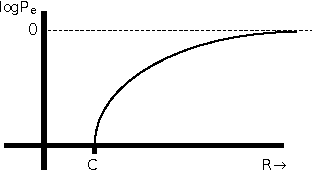
\includegraphics[width=0.5\textwidth]{images/logPe-vs-R.pdf}
                \label{fig:logPe-vs-R}
                \end{figure}

  \framebreak

  Quais os requezitos do código para que $R=C$ e $P_e = 0$?
  \begin{eqnarray}
  nR &=& H(W) = H(X^n(W)) \quad \text{\small se palavras distintas} \nonumber \\
	&=& \underbrace{H(X^n \mid Y^n)}_{=0 \text{ já que }P_e =0} + I(X^n;Y^n) = I(X^n;Y^n) \nonumber \\
	&=& H(Y^n) - H(Y^n \mid X^n) \nonumber \\
	&=& H(Y^n) - \sum_{i=1}^{n} H(Y_i \mid X_i) \nonumber \\
	&\leq& \sum_i H(Y_i) - \sum_i H(Y_i \mid X_i) \nonumber \\
	&& \text{\small com igualdade se todos $Y_i$ são ind.} \nonumber \\
	&=& \sum_i I(X_i;Y_i) \nonumber \\
	&=& nC \text{\small \ , se escolhermos $p^\ast(x) \in \argmax_{p(x)} I(X;Y)$}
  \end{eqnarray}

  \framebreak

  As condições para que $R=C$ são:
  \begin{enumerate}
  \item todas as palavras devem ser distintas;
  \item todos os $Y_i$ são independentes;
  \item a distribuição sobre $x$ é $p^\ast(x)$, uma distribuição que alcança a capacidade.
  \end{enumerate} 

\end{frame}


\subsection{Feedback}
\begin{frame}[allowframebreaks]
  \frametitle{Feedback}
  Em um canal discreto sem memória, se adicionarmos \textit{feedback} a este canal de comunicação, teremos uma taxa $R$ maior? %Seremos capazes de comunicar de forma mais eficiente?
  Mostraremos que, neste caso, a taxa não aumenta ao utilizar \textit{feedback}. 

                \begin{figure}[h!]
                \centering
                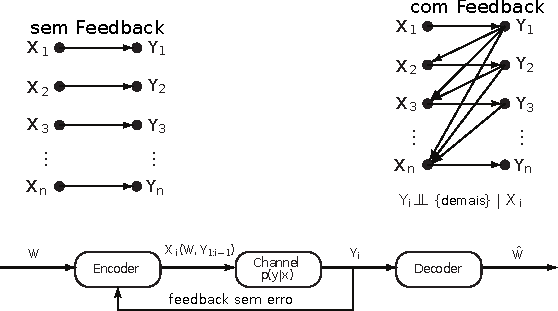
\includegraphics[width=0.6\textwidth]{images/feedback.pdf}
                \label{fig:feedback}
                \end{figure}

  \begin{itemize}
  \item O \text{feedback} pode tornar a decodificação mais simples.
  \item O \text{feedback} pode ajudar quando temos um canal com memória.
  \item No caso de um canal sem memória, \text{feedback} não ajuda a melhorar a taxa.
  \end{itemize}

  \framebreak

  \begin{definition}[código $(2^{nR}, n)$ com \textit{feedback}]
  Um código desta forma é dado por um codificador $X_i(W, Y_{1:i-1})$, um decodificador
  $g: Y^n \rightarrow \{1,2, \ldots, 2^{nR}\}$ e $P_e^{(n)} = \Pr(g(Y^n) \neq W)$ para $H(W) = nR$ (uniforme).
  \end{definition}

  \begin{definition}[Capacidade]
  A capacidade de um canal discreto sem memória com \textit{feedback} ($C_{\text{fb}}$) é o máximo de todas as taxas
  alcançáveis por códigos com \textit{feedback}.
  \end{definition}

  \framebreak

  \begin{theorem}
  \begin{equation}
  C_{\text{fb}} = C = \max_{p(x)} I(X;Y)
  \end{equation}
  para um canal discreto sem memória.
  \end{theorem}

  \begin{proof}
  \begin{itemize}
  \item $C_{\text{fb}} \geq C$, já que \textit{feedback} é uma generalização.
  \item Vamos utilizar $W$ ao invés de $X$ e limitar $R$.
  	\begin{eqnarray}
	H(W) &=& H(W \mid Y^n) + I(W;Y^n) \nonumber \\
		&\leq& 1 + P_e^{(n)} nR + I(W;Y^n) \quad \text{\small Fano}
	\end{eqnarray}
  \item Vamos limitar $I(W;Y^n)$.
  \end{itemize}

  \proofbreak

  \begin{eqnarray}
  I(W;Y^n) &=& H(Y^n) - H(Y^n \mid W) \quad \text{\small definição} \nonumber \\
	&=& H(Y^n) - \sum_{i=1}^{n} H(Y_i \mid Y_{1:i-1} , W) \quad \text{\small regra da cadeia} \nonumber \\
	&=& H(Y^n) - \sum_{i=1}^{n} H(Y_i \mid  Y_{1:i-1} , W , X_i) \quad \text{\small pois } X_i = f(W, Y_{1:i-1}) \nonumber \\
	&& Y_i \independent Y_{1:i-1} , W \mid X_i \nonumber \\
	&=& H(Y^n) - \sum_{i=1}^{n} H(Y_i \mid X_i) 
  \end{eqnarray}
  \proofbreak
  \begin{eqnarray}
  I(W;Y^n) &=& H(Y^n) - \sum_{i=1}^{n} H(Y_i \mid X_i) \nonumber \\
	&\leq& \sum_i H(Y_i) - \sum_{i=1}^{n} H(Y_i \mid X_i) \nonumber \\
	&\leq& \sum_i I(X_i;Y_i) \leq nC
  \end{eqnarray} 

  \proofbreak
  Teremos então
  \begin{equation}
  H(W) \leq 1 + P_e^{(n)} nR + nC
  \end{equation}
  e assim teremos
  \begin{equation}
  nR \leq 1 + P_e^{(n)} nR + nC
  \end{equation}
  pois a primeira desigualdade é válida para todo $H(W)$, inclusive para o máximo, quando $H(W) = nR$.
  Desta forma
  \begin{equation}
  R \leq \frac{1}{n} + P_e^{(n)} R + C
  \end{equation}
  ou $R \leq C$ quando $n \rightarrow \infty$. Então o \textit{feedback} não traz benefício.
   
  \end{proof}

\end{frame}



\subsection{Teorema Conjunto Fonte Canal}
\begin{frame}[allowframebreaks]
  \frametitle{Teorema Conjunto da Fonte/Canal}

  \begin{itemize}
  \item Compressão de dados: é possível comprimir sem erro a uma taxa média $R > H$ (bits por símbolo da fonte), 
	onde $H$ é a entropia da fonte.
  \item Transmissão de dados: é possível realizar uma comunicação sem erro se a taxa média é tal que $R < C$ 
	(bits por utilização do canal), onde $C$ é a capacidade de canal.
  \item Parece intuitivo então que seremos capazes de enviar informação de forma confiável de uma fonte com
	entropia $H$, através de um canal com capacidade $C$, se $H<C$.
  \item O canal pode ser utilizado para transmitir dados de fontes diferentes.
  \item Separação entre (de)codificador de fonte e (de)codificador de canal.
  \end{itemize}

  \framebreak
 
  \begin{itemize}
  \item Fonte: $V \in \mathcal{V}$ que satisfaz a propriedade da equipartição assintótica.
  \item Enviar $V_{1:n} = V_1, V_2, \ldots, V_n$ através de um canal.
  \item Informação por símbolo, taxa de entropia, $H(\mathcal{V})$ do processo estocástico 
	(se i.i.d., teremos $H(\mathcal{V}) = H(V_i), \forall i$).
  \item $V_{1:n} \rightarrow \text{codificador} \rightarrow  X^n \rightarrow \text{canal} \rightarrow Y^n \text{decodificador} \rightarrow \hat{V}_{1:n}$
  \item probabilidade de erro:
	\begin{eqnarray}
	P_e^{(n)} &=& P(V_{1:n} \neq \hat{V}_{1:n}) \\
		&=& \sum_{y_{1:n}} \sum_{v_{1:n}} \Pr(v_{1:n}) \Pr(y_{1:n} \mid X^n( v_{1:n} )) \mathbf{1}_{\{ g(y_{1:n}) \neq v_{1:n} \}} \nonumber
	\end{eqnarray}
  \end{itemize}
  \framebreak

  \begin{theorem}[Teorema da Codificação de Fonte/Canal]
  Se $V_{1:n}$ é um processo estocástico com alfabeto finito que satisfaz a prop. da eq. ass.
  e $H(\mathcal{V}) < C$,  então $\exists$ uma sequência de códigos $(2^{nR},n)$ com
  $P_e^{(n)} \rightarrow 0$. Por outro lado, se $H(\mathcal{V}) > C$,
  então $P_e^{(n)} > 0$ para qualquer $n$ e não será possível enviar informação com 
  probabilidade de erro arbitrariamente pequena.
  \end{theorem}

  \framebreak
  \begin{proof}
  \begin{itemize}
  \item Se $V$ satisfaz a prob. da eq. ass., então $\exists$ um conjunto $A_{\epsilon}^{(n)}$ 
	com $\vert A_{\epsilon}^{(n)} \vert \leq 2^{n(H(\mathcal{V}) + \epsilon)}$, e neste conjunto
	está contido `tudo' aquilo que ocorre.
  \item Iremos codificar apenas o conjunto típico e enviar um erro caso contrário.
	Isto contribui em, no máximo, $\epsilon$ para a $P_e$.
  \item Vamos indexar os elementos de $A_{\epsilon}^{(n)}$ com $\{1,2,\ldots,2^{n(H+\epsilon)}\}$, 
	precisaremos então de $n(H+\epsilon)$ bits.
  \item A taxa será $R = H(\mathcal{V}) + \epsilon$. Se $R < C$ então a probabilidade de erro 
	será menor que $\epsilon$, e poderemos fazê-la tão pequena quanto desejado.
  \end{itemize}

  \proofbreak

  \begin{eqnarray}
  P_e^{(n)} &=& \Pr(V_{1:n} \neq \hat{V}_{1:n}) \nonumber \\
		&\leq& \Pr(V_{1:n} \notin A_{\epsilon}^{(n)}) + \underbrace{ \Pr(g(Y^n) \neq V^n \mid V^n \in A_{\epsilon}^{(n)} ) }_{< \epsilon , \text{ já que } R < C} \nonumber \\
		&\leq& \epsilon + \epsilon = 2 \epsilon
  \end{eqnarray}
  É possível assim reconstruir a sequência com baixa probabilidade de erro para $n$ grande suficiente, se
  \begin{equation}
  H(\mathcal{V}) < C .
  \end{equation}
  \end{proof}

  \framebreak
  \begin{proof}[proposição inversa]
  \begin{itemize}
  \item Para mostrar que $P_e^{(n)} \rightarrow 0 \Rightarrow H(\mathcal{V}) \leq C$ iremos definir
	\begin{equation}
	\text{codificador: } X^n(V^n): \mathcal{V}^n \rightarrow \mathcal{X}^n
	\end{equation} 
        \begin{equation}
        \text{decodificador: } g(Y^n): \mathcal{Y}^n \rightarrow \mathcal{V}^n
        \end{equation} 
  \item Fano: $H(X\mid Y) \leq 1 + P_e \log \vert \mathcal{X} \vert$.
  \item Teremos então:
	\begin{equation}
	H(V^n \mid \hat{V}^n) \leq 1 + P_e^{(n)} \log \vert \mathcal{V}^n \vert = 1  + n P_e \log \vert \mathcal{V} \vert
	\end{equation}
  \end{itemize}

  \proofbreak

	\begin{eqnarray}	
	H(\mathcal{V}) &\leq& \frac{H(V_1, V_2, \ldots, V_n)}{n} = \frac{H(V_{1:n})}{n} \nonumber \\
		&=& \frac{1}{n} H(V_{1:n} \mid \hat{V}_{1:n}) + \frac{1}{n} I(V_{1:n};\hat{V}_{1:n}) \nonumber \\
		&& \text{\small Fano} \nonumber \\
		&\leq& \frac{1}{n} (1 +  P_e^{(n)} n \log \vert \mathcal{V} \vert) + \frac{1}{n} I(V_{1:n};\hat{V}_{1:n}) \nonumber \\
		&& \text{\small desig. proc. dados } V \rightarrow X \rightarrow Y \rightarrow \hat{V} \nonumber \\
		&\leq& \frac{1}{n} (1 +  P_e^{(n)} n \log \vert \mathcal{V} \vert) + \frac{1}{n} I(X_{1:n}; Y_{1:n}) 
	\end{eqnarray}

  \proofbreak

	\begin{eqnarray}        
        H(\mathcal{V}) &\leq& \frac{1}{n} (1 +  P_e^{(n)} n \log \vert \mathcal{V} \vert) + \frac{1}{n} I(X_{1:n}; Y_{1:n}) \nonumber \\
			&& \text{\small otimização capacidade, sem memória} \nonumber \\
			&\leq& \frac{1}{n} + P_e^{(n)} \log \vert \mathcal{V} \vert + C
	\end{eqnarray}

  Fazendo $n \rightarrow \infty$, teremos $1/n \rightarrow 0$ e $P_e \rightarrow 0$, assim obtemos $H(\mathcal{V}) \leq C$.
  \end{proof}


\end{frame}


\subsection{Exercícios}
\begin{frame}[allowframebreaks]
  \frametitle{Canal Binário com Apagamento}
  3 formas de calcular a capacidade do canal binário com apagamento
  \begin{exercise}[Capacidade do canal binário com apagamento]
  Considere o canal binário com apagamento ilustrado abaixo.
      \begin{figure}[h!]
      \centering
      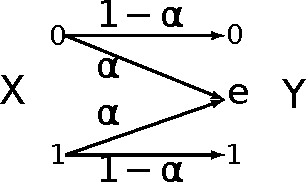
\includegraphics[width=0.2\textwidth]{images/bech.pdf}
      \label{fig:bechrev}
      \end{figure}
  A capacidade do canal é dada por:
  \begin{equation}
  C = \max_{p(x)} I(X;Y) = \max_{p(x)} H(X) - H(X|Y) = \max_{p(x)} H(Y) - H(Y|X)
  \end{equation}
  Podemos adotar dois caminhos, usando $H(X) - H(X|Y)$ ou $H(Y) - H(Y|X)$.
  
  \exercisebreak
  Calcular $H(X)$ depende apenas de $p(x)$, teremos $H(X) = H(p)$.

  Para calcular $H(X|Y)$ devemos analisar cada uma das possíveis saídas:
  \begin{eqnarray}
  H(X|Y) &=& \sum_y p(y) H(X|Y=y) \\
	&=& p(Y=0) \underbrace{H(X|Y=0)}_{=0} + \underbrace{p(Y=e)}_{=\alpha} \underbrace{H(X|Y=e)}_{=H(p)} + \nonumber \\
	&& p(Y=1) \underbrace{H(X|Y=1)}_{=0} \nonumber \\
	&=& \alpha H(p)
  \end{eqnarray}
  \exercisebreak
  Logo, teremos $I(X;Y) = H(p) - \alpha H(p) = (1-\alpha) H(p)$.
  \begin{equation}
  C = \max_{p} (1-\alpha) H(p) = (1-\alpha) ,
  \end{equation}
  onde a distribuição $p$ que maximiza é a uniforme $p = (0.5, 0.5)$.

  \exercisebreak
  Para o segundo caminho deveremos calcular $H(Y)$ e $H(Y|X)$.
  O cálculo de $H(Y|X)$ é simples:
  \begin{eqnarray}
  H(Y|X) &=& \sum_x p(x) H(Y|X=x) \nonumber \\
	&=& p_0 \underbrace{H(Y|X=0)}_{=H(\alpha)} + p_1 \underbrace{H(Y|X=1)}_{=H(\alpha)} \nonumber \\
	&=& H(\alpha) .
  \end{eqnarray}
  \exercisebreak
  Para calcular $H(Y)$ podemos calcular as probabilidades de $Y=0$, $Y=e$ e $Y=1$, e então calcular
  \begin{eqnarray} 
   H(Y) &=& H(\Pr(Y=0),\Pr(Y=e),\Pr(Y=1)) , \nonumber \\ 
        &=& H \left( p_0 (1-\alpha) , \alpha, p_1 (1-\alpha) \right)
  \end{eqnarray}
  conforme feito anteriormente (ver slide \ref{sldbech}).

  \exercisebreak

  Ou ainda, podemos ver que a determinação de $Y$ pode ser quebrada em duas etapas: 1) houve apagamento ou não 
  (entropia associada a esta etapa é $H(\alpha)$);
  2) caso não tenha ocorrido apagamento (o que ocorre com probabilidade $1-\alpha$), $Y$ será $0$ ou $1$ 
  (entropia associada a esta etapa é $H(p)$.

     \begin{figure}[h!]
     \centering
     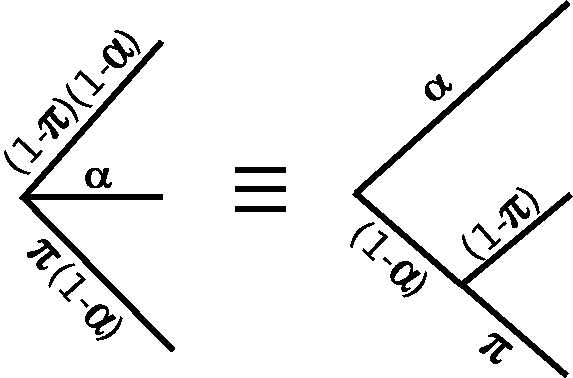
\includegraphics[width=0.3\textwidth]{images/eqvh.pdf}
     \label{fig:eqvh2}
     \end{figure}

  \exercisebreak
  Teremos assim que
  \begin{equation}
  H(Y) = H(\alpha) + (1-\alpha) H(p).
  \end{equation}
  Desta forma, teremos
  \begin{eqnarray}
  C &=& \max_{p(x)} I(X;Y) = \max_{p(x)} H(Y) - H(Y|X) \nonumber \\
	&=& \max_{p(x)} H(\alpha) + (1-\alpha) H(p) - H(\alpha) \nonumber \\
	&=& \max_{p(x)} (1-\alpha) H(p) = 1-\alpha ,
  \end{eqnarray}
  onde a distribuição $p$ que maximiza é a uniforme $p = (0.5, 0.5)$.

  \end{exercise}
\end{frame}


\begin{frame}[allowframebreaks]
  \frametitle{Capacidade de Canal}
  % ee/ufsj/2014_02/ti/aula/radford/ass3-sol.pdf

  \begin{exercise}[Capacidade de Canal]
  Considere um canal discreto em que os alfabetos de entrada e saída são 
  $\mathcal{X} = \mathcal{Y} = \{0,1,2\}$. As probabilidades de transição 
  para este canal são dadas: $p(y=0 | x=0) = p(y=2 | x=2) = 1$, 
  $p(y=0 | x=1) = p(y=2 | x=1) = 1/4$ e $p(y=1 | x=1)=1/2$.

  \exercisebreak

  \begin{enumerate}[a)]
  \item Ache a informação mútua entre a entrada do canal e a saída se as probabilidades
  da entrada são dadas por $p(x=0)=1/2$, $p(x=1)=0$ e $p(x=2)=1/2$.

  \textit{(solução)}

  \begin{equation}
  I(X;Y) = \underbrace{H(X)}_{=1} - \underbrace{H(X|Y)}_{= 0} = 1
  \end{equation}
  onde utilizamos que, dado $Y$, como $y=1$ não ocorre, então não existe incerteza
  sobre $X$, uma vez que sendo enviado $0$ ou $2$, iremos receber o mesmo símbolo.
  \end{enumerate}

  \exercisebreak

  \begin{enumerate}[b)]
  \item Encontre a informação mútua entre a saída e entrada no canal quando a probabilidade
  da entrada é uniforme.
  \end{enumerate}

  \textit{(solução)}

  $I(X;Y) = H(Y) - H(Y|X)$. 
  Vamos calcular então as probabilidades das saídas
  $p(y=0) = p(x=0) + (1/4) p(x=1) = 5/12$; 
  $p(y=1) = (1/2) p(x=1) = 1/6$; e
  $p(y=2) = p(x=2) + (1/4)p(x=1) = 5/12$.
  \exercisebreak

  \begin{equation}
  H(Y) = \frac{5}{12} \log \frac{12}{5} + \frac{1}{6} \log 6 + \frac{5}{12} \log \frac{12}{5} = 1.483
  \end{equation}
  \vspace{-1em}
  \begin{eqnarray}
  H(Y|X) &=& \frac{1}{3} \underbrace{H(Y | X=0)}_{=0} + \frac{1}{3} H(Y | X=1) + \frac{1}{3} \underbrace{H(Y | X=2)}_{=0} \nonumber \\
         &=& \frac{1}{3} H(Y | X=1) \nonumber \\
	&=& \frac{1}{3} \left[ \frac{1}{4} \log 4 + \frac{1}{2} \log 2 + \frac{1}{4} \log 4 \right] = \frac{1}{3} \times \frac{3}{2} = \frac{1}{2}
  \end{eqnarray}
  \exercisebreak
 
  e assim a informação é dada por
  \begin{equation}
  I(X;Y) = H(Y) - H(Y|X) = 1.483 - 0.5 = 0.983 \text{ bits}.
  \end{equation}

  \exercisebreak

  \begin{enumerate}[c)]
  \item Encontre a capacidade destes canal e uma distribuição para a entrada capaz de atingir esta capacidade.
  \end{enumerate}

  \textit{(solução)}
  
  Queremos maximizar $I(X;Y)$ com relação a $p_0, p_1, p_2$ ($p(x=0), p(x=1), p(x=2)$, respectivamente),
  que devem ser positivos e somar $1$. Vamos chamar de $q_0 = p(y=0)$, $q_1 = p(y=1)$ e $q_2 = p(y=2)$.

  Temos então: $q_0 = p_0 + (1/4)p_1$, $q_1 = (1/2) p_1$ e $q_2 = p_2 + (1/4) p_1$.

  Iremos mostrar que $I(X;Y)$ poderá ser maximizada quando a distribuição de entrada for tal que $p_0=p_2$.
  
  \exercisebreak

  Podemos escrever $p_2 = 1 - p_1 - p_0$.

  As probabilidades de saída serão $q_0 = p_0 + (1/4) p_1$, $q_1 = (1/2) p_1$ e $q_2 = p_2 + (1/4)p_1$.

  $I(X;Y) = H(Y) - H(Y|X)$. Note que $H(Y|X) = p_1 H(Y|X=1)$ e, desta forma, depende apenas de $p_1$.
  Dado um valor para $p_1$, teremos $q_1$ determinado e assim $H(Y)$ será maximizado quando $q_0$ e $q_2$
  forem iguais, o que irá ocorrer quando $p_0 = p_2$. Logo, fixando $p_1$, o máximo de $I(X;Y)$ será alcançado
  quando $p_0 = p_2 = (1-p_1)/2$. Para este valor de $p_0$ e $p_2$, teremos $q_0 = q_2 = (2-p_1)/4$.

  \exercisebreak

  Teremos assim
  \begin{eqnarray}
  H(Y) 	&=& -q_0 \log q_0 - q_1 \log q_1 - q_2 \log q_2 \nonumber \\
	&=& - 2 \left( (2-p_1)/4 \log (2-p_1)/4 \right) - (p_1/2) \log (p_1/2) 
  \end{eqnarray}

  A informação mútua para $p_0 = p_2$ será dada por
  \begin{equation}
  I(X;Y) = - (1-p_1/2) \log ((2-p_1)/4) - (p_1/2) \log (p_1/2) - (3/2) p_1
  \end{equation}

  \exercisebreak

  \lstinputlisting[language=Matlab,basicstyle=\footnotesize]{exercicios/exmpl-max-i.m}
%  \begin{lstlisting}
%  p1 = [0.001 : 0.001 : 0.999];
%  I = -(1-p1/2).*log2((2-p1)/4) - (p1/2).*log2(p1/2) - (3/2)*p1;
%  plot(p1,I); xlabel('p1'); ylabel('I(X;Y)');
%  [mI, id] = max(I);
%  p1(id)
%  ans =  0.11800
%  \end{lstlisting}

  O máximo ocorrerá quando $p_1 = 0.118$ e $p_0 = p_2 = 0.441$.

  \exercisebreak

  \begin{figure}[h!]
  \centering
  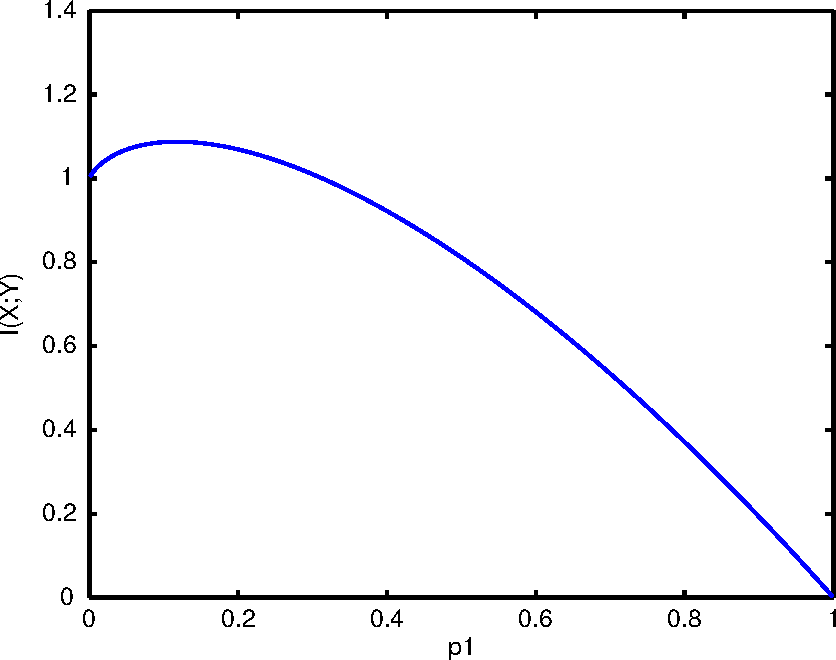
\includegraphics[width=0.4\textwidth]{images/exmpl-max-i.pdf}
  \label{fig:exmpl-max-i}
  \end{figure}

  %  \exercisebreak
  \end{exercise}
  
\end{frame}

\begin{frame}[allowframebreaks]
  \frametitle{Canal da Soma}
  % ~/ee/ufsj/2015_02/ti/provas/midterm2_2009_solutions.pdf
  \begin{exercise}[Canal da Soma]
  %  \exercisebreak
  Seja $\mathcal{X} = \mathcal{Y} = \{A,B,C,D\}$ os alfabetos de entrada e saída de um
  canal discreto sem memória com probabilidades de transição $p(y|x)$ dadas pela matriz abaixo,
  para $0 \leq \epsilon , \delta \leq 1$,

  \begin{equation}
  p(y|x) = 
  \begin{pmatrix}
  1-\epsilon & \epsilon & 0 & 0 \\
  \epsilon & 1-\epsilon & 0 & 0 \\
  0 & 0 & 1 - \delta & \delta \\
  0 & 0 & \delta & 1 - \delta
  \end{pmatrix}
  \end{equation}

  \exercisebreak

  Note que este canal com 4 entradas e saídas equivale à soma ou união de dois canais
  em paralelo com matrizes de transição dadas por

  \noindent\begin{minipage}{.5\linewidth}
  \begin{equation}
  p_1(y|x) = \begin{pmatrix} 1-\epsilon & \epsilon \\ \epsilon & 1-\epsilon \end{pmatrix}
  \end{equation}
  \end{minipage}%
  \begin{minipage}{.5\linewidth}
  \begin{equation} 
  p_2(y|x) = \begin{pmatrix}  1 - \delta & \delta \\ \delta & 1 - \delta \end{pmatrix}
  \end{equation}
  \end{minipage}

  %\doubleequation[eq:p1-canal1,eq:p2-canal2]{p_1(y|x) = \begin{pmatrix} 1-\epsilon & \epsilon \\ \epsilon & 1-\epsilon \end{pmatrix}}{p_2(y|x) = \begin{pmatrix}  1 - \delta & \delta \\ \delta & 1 - \delta \end{pmatrix}  }
  com alfabetos $\mathcal{X}_1 = \mathcal{Y}_1 = \{A,B\}$ 


  \exercisebreak
  
  \begin{enumerate}[a)]
  \item Esboce o diagrama de transições deste canal.
  \end{enumerate}
  \textit{(solução)}

  \begin{figure}[h!]
  \centering
  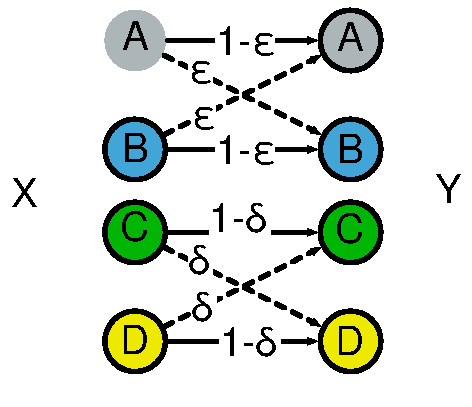
\includegraphics[width=0.2\textwidth]{images/pchannel.pdf}
  \label{fig:pchannel}
  \end{figure}


  \exercisebreak

  \begin{enumerate}[b)]
  \item Encontre a capacidade do canal para $\epsilon = \delta = 1/2$.
  \end{enumerate}
  \textit{(solução)}

  Nesta situação ($\epsilon = \delta = 1/2$) temos uma canal simétrico, e sua capacidade
  é alcançada por uma distribuição uniforme. A capacidade será dada por
  \begin{eqnarray}
  C &=& \log \vert \mathcal{Y} \vert - H(r) \\
	&& \text{onde } r \text{ é uma linha da matriz de transição} \nonumber \\
	&=& \log 4 - H(\frac{1}{2}, \frac{1}{2}, 0, 0) \nonumber \\
	&=& 2 - 1 = 1 \text{ (bit por utilização do canal)} \nonumber
  \end{eqnarray}   

  \exercisebreak

  \begin{enumerate}[c)]
  \item Seja $p(x)$ uma função massa probabilidade em $\mathcal{X}$ e seja
  $p(A)+p(B) = \alpha$ e $p(C)+p(D)=1-\alpha$.
  Mostre que a informação mútua entre $X$ e $Y$ poderá ser expressa por
  \begin{equation}
  I(X;Y) = H(\alpha) + \alpha I(X;Y | X \in \{A,B\}) + (1-\alpha) I(X;Y|X \in \{C,D\}).
  \end{equation}
  \end{enumerate}
  \textit{(solução)}
  Vamos definir uma v.a. $\theta \in \{0,1\}$ tal que, 
  $x \in \{A,B\} \Rightarrow \theta = 1$ e 
  $x \in \{C,D\} \Rightarrow \theta = 0$, logo a função massa de probabilidade de $\theta$
  será dada por
  \begin{equation}
  p_\theta = \begin{cases} \alpha, \quad \theta = 1  \\ 1-\alpha, \quad \theta = 0 \end{cases}
  \end{equation}

  \exercisebreak
  A informação mútua entre $X$ e $Y$ poderá ser expressa como
  \begin{eqnarray}
  I(X;Y) &=& I(X; \theta) + I(X;Y|\theta) \nonumber \\
	&=& H(\theta) - H(\theta | X) + I(X;Y|\theta) \nonumber \\
	&=& H(\alpha) - 0 + p(\theta=1) I(X;Y|\theta=1) + p(\theta=0) I(X;Y | \theta = 0) \nonumber \\
	&=& H(\alpha) + \alpha I(X;Y|X\in\{A,B\}) + (1-\alpha) I(X;Y|X\in\{C,D\})
  \end{eqnarray}


  \exercisebreak
  \begin{enumerate}[d)]
  \item Seja $C_1$ e $C_2$ as capacidades dos canais descritos por $p_1(y|x)$ e $p_2(y|x)$.
  Mostre que 
  	\begin{equation}
	\max_{p(x)} I(X;Y) = \max_{\alpha} \left( H(\alpha) + \alpha C_1 +(1-\alpha) C_2 \right)
	\end{equation}
  \end{enumerate}
  \textit{(solução)}

  Note que 
  \noindent\begin{minipage}{.5\linewidth}
  \begin{equation}
  C_1 = \max_{p_1(x) : x\in\{A,B\}} I(X;Y) 
  \end{equation}
  \end{minipage}%
  \begin{minipage}{.5\linewidth}
  \begin{equation} 
  C_2 = \max_{p_2(x):x\in\{C,D\}} I(X;Y)
  \end{equation}
  \end{minipage}
 
  \exercisebreak

  Como $x \in \{A,B\} \rightarrow y \in \{A,B\}$ e $x \in \{C,D\} \rightarrow y \in \{C,D\}$,
  teremos 
  \begin{eqnarray}
  \max_{p(x):x\in\{A,B,C,D\}} I(X;Y) &=& \nonumber \\
	\max_{p(x):x\in\{A,B,C,D\}, 0\leq \alpha \leq 1} 
	\left( H(\alpha) + \alpha I(X;Y|X\in\{A,B\}) + \right.  && \nonumber \\ \left. (1-\alpha) I(X;Y|X\in\{C,D\}) \right) &=& \nonumber \\
	\max_{0\leq \alpha \leq 1} \left( H(\alpha) + 
		\max_{p(x):x\in\{A,B\}} \alpha I(X;Y | X \in \{A,B\}) + \right.  && \nonumber \\ \left. 
		\max_{p(x):x\in\{C,D\}} (1-\alpha) I(X;Y | X \in \{C,D\}) \right) &=& \nonumber \\
	 \max_{0\leq \alpha \leq 1} \left( H(\alpha) + \alpha C_1 + (1-\alpha) C_2 \right)
  \end{eqnarray}


  \exercisebreak
  \begin{enumerate}[e)]
  \item Encontre a capacidade $C$ do canal de soma em termos das capacidades $C_1$ e $C_2$
  dos sub-canais, sem utilizar outros parâmetros.
  \end{enumerate}
  \textit{(solução)}

  Utilizando o resultado do item anterior fica mais fácil. 
  Poderemos então utilizar a capacidade dos canais binários simétricos 
  $C_1 = 1 - H(\epsilon)$ e $C_2 = 1 - H(\delta)$.
  Desta forma, definimos uma função $f(\alpha) := H(\alpha) + \alpha C_1 + (1-\alpha) C_2$,
  a qual queremos maximizar com relação ao parâmetro $\alpha$. Teremos então um problema
  de otimização unidimensional. Devemos encontrar o ponto em que a derivada primeira 
  se igual a zero, quando a derivada segunda é negativa.

  \exercisebreak

  \begin{eqnarray}
  \frac{d f(\alpha)}{d \alpha} &=& H'(\alpha) + C_1 - C_2 \nonumber \\
	&=& \frac{1}{\ln 2} \ln \left( \frac{1-\alpha}{\alpha} \right) + \frac{1}{\ln 2} C_1 - \frac{1}{\ln 2} C_2 \nonumber \\
	&=& \log \left( \frac{1-\alpha}{\alpha} \right) + C_1 - C_2
  \end{eqnarray}

  \exercisebreak
  \begin{eqnarray}
  \frac{d^2 f(\alpha)}{d \alpha^2} &=& \frac{1}{\ln 2} \frac{\alpha}{1 - \alpha} \frac{- \alpha - 1 + \alpha}{\alpha^2} \nonumber \\
	&=& \frac{1}{\ln 2} \frac{1}{\alpha - 1}
  \end{eqnarray}
  como $0 \leq \alpha \leq 1$, teremos que $\frac{d^2 f(\alpha)}{d \alpha^2} < 0$, logo o ponto que 
  encontraremos quando $\frac{d f(\alpha)}{d \alpha} = 0$ será um ponto de máximo.

  \exercisebreak

  \vspace{-1em}
  O ponto de máximo será então dado por
  \begin{eqnarray}
  \log \left( \frac{1-\alpha}{\alpha} \right) + C_1 - C_2 &=& 0 \nonumber \\
  \log \left( \frac{1-\alpha}{\alpha} \right) &=& C_2 - C_1 \nonumber \\
  \frac{1-\alpha}{\alpha} &=& \frac{2^{C_2}}{2^{C_1}} \nonumber \\
  \alpha 2^{C_2} &=& (1-\alpha) 2^{C_1} \nonumber \\
  \alpha (2^{C_1} + 2^{C_2}) &=& 2^{C_1} \nonumber \\
  \alpha &=& \frac{2^{C_1}}{2^{C_1} + 2^{C_2}}
  \end{eqnarray}

  \exercisebreak
  Substituindo o valor encontrado para $\alpha$, teremos
  \begin{eqnarray}
  C &=& H(\alpha) + \alpha C_1 + (1 - \alpha) C_2 \nonumber \\
	&=& -\alpha \log \alpha - (1 - \alpha) \log (1 - \alpha) + \alpha C_1 + (1 - \alpha) C_2 \nonumber \\
	&=& \alpha (C_1 - C_1 + \log (2^{C_1} + 2^{C_2}) + (1-\alpha)(C_2 - C_2 + \log(2^{C_1}-2^{C_2})) \nonumber \\
	&=& \alpha \log (2^{C_1} + 2^{C_2}) + (1 - \alpha) \log (2^{C_1} + 2^{C_2}) \nonumber \\
	&=& \log (2^{C_1} + 2^{C_2}) 
  \end{eqnarray}   
  \end{exercise}

\end{frame}


\begin{frame}[allowframebreaks]
  \frametitle{Canais em Cascata com Codificador}
  % ~/ee/ufsj/2015_02/ti/provas/midterm2_2009_solutions.pdf
  \begin{exercise}[Canais em cascata com codificador entre eles]

  Considere a canais binários simétricos conectados em cascata com um codificador entre
  eles, conforme ilustrado abaixo. Calcule a capacidade do canal entre $X$ e $Y$.
  \begin{figure}[h!]
  \centering
  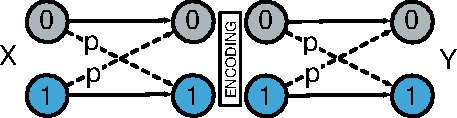
\includegraphics[width=0.5\textwidth]{images/c-enc-c.pdf}
  \label{fig:c-enc-c}
  \end{figure}

  \exercisebreak
  \textit{(solução)}

  Os símbolos são re-codificados após o primeiro canal, desta forma a 
  capacidade torna-se $C = \min (C_1, C_2)$, onde $C_1$ e $C_2$ são as
  capacidades do primeiro e segundo canais binários, respectivamente.
  Como neste caso os canais são iguais, temos $C_1 = C_2 = 1 - H(p)$.
  Logo, a capacidade do canal será $C = 1 - H(p)$, sendo este valor alcançado
  quando a distribuição de $X$ for uniforme.
 
  \end{exercise}
\end{frame}


\begin{frame}[allowframebreaks]
  \frametitle{Canal Z}
  % ~/ee/ufsj/2015_02/ti/provas/midterm2_2010_solutions.pdf
  \begin{exercise}[Canal Z]
  Considere o canal Z, com capacidade $C_Z$, ilustrado abaixo. Considere
  a seguinte distribuição de entrada: $p(X=0) = q$, $p(X=1)=1-q$.
  Encontre a equação que deverá ser otimizada para encontrarmos a capacidade deste canal
  (simplifique a equação ao máximo, mas não é necessário solucioná-la).
  \begin{figure}[h!]
  \centering
  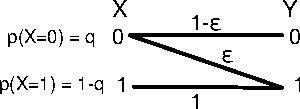
\includegraphics[width=0.4\textwidth]{images/canalz.pdf}
  \label{fig:canalz}
  \end{figure}

  obs.: as características de erro em sistemas ópticos e memória de alguns
	  semi-condutores podem ser modeladas através de um canal z.

  \exercisebreak
  \textit{(solução)}

  Devemos encontrar $q$ que maximiza $I(X;Y) = H(Y) - H(Y|X)$. Primeiramente iremos
  encontrar uma expressão para $I(X;Y)$ em termos de $q$ e $\epsilon$. Vamos tomar
  a derivada com relação a $q$ e achar o $q$ que faz com que esta derivada seja igual a zero.

  Note que $p(Y=0) = q(1-\epsilon)$ e, por conseguinte, $p(Y=1) =1 - q(1-\epsilon)$, assim,
  $H(Y) = H( q(1-\epsilon) )$.
  \exercisebreak
  \vspace{-2em}
  \begin{eqnarray}
  I(X;Y) &=& H(Y) - H(Y|X) \nonumber \\
	&=& H( q(1-\epsilon) ) + (1-q) \underbrace{H(Y|X=1)}_{=0} + q \underbrace{H(Y|X=0)}_{=H(\epsilon)} \nonumber \\
	&=& H( q(1-\epsilon) ) + q H(\epsilon) \nonumber \\
	&=& -q(1-\epsilon) \log q (1-\epsilon) - (1 - q(1-\epsilon)) \log (1 - q(1-\epsilon)) + \nonumber \\
	&& q H(\epsilon)
  \end{eqnarray}
  Devemos tomar $\frac{d I(X;Y)}{dq} = 0$ e achar $q$ que satisfaz esta equação.

  \exercisebreak

  \begin{equation}
  C \approx 1 - \frac{1}{2} H(\epsilon)
  \end{equation}
  que será alcançada quando
  \begin{equation}
	  q = \frac{1}{(1-\epsilon)(1+2^{\nicefrac{H(\epsilon)}{(1-\epsilon)}})}
  \end{equation}

%  \exercisebreak

%  \begin{eqnarray}
%  \frac{ \partial I(X;Y)}{\partial q} &=& -(1-\epsilon) \log q (1-\epsilon) - q (1-\epsilon) \frac{1}{q (1-\epsilon)} + H(\epsilon) \\
%	&=& -(1-\epsilon) \log q (1-\epsilon) - 1 + H(\epsilon) = 0
%  \end{eqnarray}

%  \exercisebreak

%  \begin{eqnarray}
%  \log q (1-\epsilon) &=& \frac{H(\epsilon) - 1}{1-\epsilon} \\
%  q (1-\epsilon) &=& 2^{\frac{H(\epsilon) - 1}{1-\epsilon}} \\
%  q &=& \frac{2^{\frac{H(\epsilon) - 1}{1-\epsilon}}}{1-\epsilon}
%  \end{eqnarray}
  \end{exercise}


  \framebreak

  \begin{exercise}[Canal Z em cascata]
  Considere agora a cascata de dois canais Z, conforme ilustrado na figura abaixo.
  \begin{figure}[h!]
  \centering
  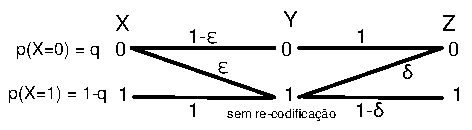
\includegraphics[width=0.55\textwidth]{images/canalzc.pdf}
  \label{fig:canalzc}
  \end{figure}
  A saída de um canal é inserida diretamente no canal seguinte, sem recodificação.
  Encontre as probabilidades de transição do canal final criado pela cascata dos
  2 canais Z.
 
  \exercisebreak 
  \begin{enumerate}[a)]
  \item Encontre as probabilidades de transição para o canal final (entre $X$ e $Z$).
  \end{enumerate}
  \textit{(solução)}
  
  O canal efetivo entre $X$ e $Z$ é descrito pelas probabilidades
  \begin{equation}
  p(Z=0|X=0) = (1-\epsilon) + \epsilon \delta
  \end{equation}
  \begin{equation}
  p(Z=1|X=0) = \epsilon (1-\delta)
  \end{equation}
  \begin{equation}
  p(Z=0|X=1) = \delta
  \end{equation}
  \begin{equation}
  p(Z=1|X=1) = 1-\delta
  \end{equation}

  \exercisebreak

  \begin{equation}
  p(z|x) = 
    \begin{pmatrix}
    (1-\epsilon) + \epsilon \delta & \epsilon (1-\delta) \\
    \delta 	& 1-\delta
    \end{pmatrix}
  \end{equation}

  \exercisebreak
    
  \begin{enumerate}[b)]
  \item Encontre o valor de $\delta$ (em termos de $\epsilon$) que faz com que o canal final $XZ$
  seja simétrico e encontre a capacidade deste canal $C_{XZ}$.
  \end{enumerate}
  \textit{(solução)}

  Devemos ter $p(Z=1|X=0) = p(Z=0|X=1)$, ou seja,
  \begin{equation}
  \epsilon = \frac{\delta}{1-\delta}
  \end{equation}
  Note que esta escolha levará também a $p(Z=1|X=1) = p(Z=0|X=0)$.

  \exercisebreak

  Como o canal é simétrico, teremos
  \begin{eqnarray}
  C &=& \log \vert \mathcal{Z} \vert - H(r) \nonumber \\
	&=& \log 2 - H(\delta) \nonumber \\
	&=& 1 - H(\delta).
  \end{eqnarray} 
  onde $r$ é uma linha da matriz de transição, ou seja, $r = [\delta \quad (1-\delta)]$, utilizando 
  $\epsilon = \delta / (1 - \delta)$.

  \exercisebreak
  \begin{enumerate}[c)]
  \item Considere agora que, em $Y$, seja possível decodificar e recodificar a sequência recebida.
  Qual é a capacidade do sistema agora?
  \end{enumerate}
  \textit{(solução)}

  \begin{equation}
  C = \min (C_Z , C_{YZ}) .
  \end{equation}
  onde $C_Z$ é a capacidade do canal $X \text{\textemdash} Y$ e $C_{YZ}$ é a capacidade do canal $Y \text{\textemdash} Z$.
  \end{exercise}
\end{frame}


\begin{frame}[allowframebreaks]
  \frametitle{Sequencias Típicas}
  \begin{exercise}[Sequencias Típicas]
  Vamos calcular o conjunto de pares de variáveis aleatórias conjuntamente típicas e conectadas 
  através de um canal binário simétrico e a probabilidade de erro para a decodificação 
  através da tipicidade conjunta para este canal.

  \begin{figure}[h!]
  \centering
  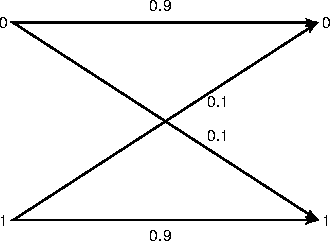
\includegraphics[width=0.3\textwidth]{images/ex715channel.pdf}
  \label{fig:ex715channel}
  \end{figure}

  \examplebreak
  Vamos considerar um canal binário simétrico com probabilidade de troca de bit de $0.1$.
  A distribuição de entrada que atinge o limite da capacidade é a distribuição uniforme,
  i.e., $p(x) = (1/2, 1/2)$, que leva à seguinte distribuição conjunta $p(x,y)$ para
  este canal:

  \begin{tabular}{c|cc}
  $X \setminus Y$ & 0 & 1 \\ \hline
  0  & 0.45 & 0.05 \\
  1  & 0.05 & 0.45
  \end{tabular}

  A distribuição marginal de $Y$ também será $(1/2, 1/2)$.

  \examplebreak
  \begin{enumerate}[a)]
  \item Calcule $H(X)$, $H(Y)$, $H(X,Y)$ e $I(X;Y)$ para a distribuição dada.
  \end{enumerate}
 
  \textit{(solução)}

  $H(X) = H(Y) = 1$ bit já que ambos possuem distribuição $(1/2, 1/2)$.
  $H(X,Y) = H(X) + H(Y|X) = 1 + H(p) = 1 - 0.9 \log 0.9 - 0.1 \log 0.1 = 1 + 0.469 = 1.469$ bits.
  $I(X;Y) = H(Y) - H(Y|X) = 1 - 0.469 = 0.531$ bits.
 

  \examplebreak
  \begin{enumerate}[b)]
  \item Sejam $X_1, X_2, \ldots, X_n$, i.i.d. com distribuição de Bernoulli$(1/2)$.
  Dentre as $2^n$ possíveis sequências de entrada de comprimento $n$, quais delas são típicas,
  i.e., membros de $A_\epsilon^{(n)}(X)$ para $\epsilon = 0.2$? Quais são as sequências
  típicas em $A_\epsilon^{(n)}(Y)$?
  \end{enumerate}
  
  \textit{(solução)}

  No caso em que a distribuição é uniforme, toda sequência terá a mesma probabilidade $(1/2)^n$ 
  e, desta forma, para toda sequencia, $-\frac{1}{n} \log p(x^n) = -\frac{1}{n} n \log 1/2 = 1 = H(X)$.
  Desta forma teremos que toda sequência é típica, i.e. $\in A_{\epsilon}^{(n)}$.

  De forma semelhante, toda sequência $y^n$ é típica, i.e., $\in A_\epsilon^{(n)}(Y)$.

  \examplebreak
  \begin{enumerate}[c)]
  \item O conjunto das sequências conjuntamente típicas $A_\epsilon^{(n)}(X,Y)$ é definido
  pelo conjunto das sequências que satisfazem a Equação \ref{eq-tipicidade-conjunta}.
  As duas primeiras equações correspondem à condição que $x^n$ e $y^n$ estejam em
  $A_\epsilon^{(n)}(X)$ e $A_\epsilon^{(n)}(Y)$ respectivamente. Considere a última condição,
  que pode ser reescrita da seguinte forma: 
  $-\frac{1}{n} \log p(x^n, y^n) \in \left( H(X,Y) - \epsilon, H(X,Y) + \epsilon \right)$.
  Seja $k$ o número de lugares em que a sequência $x^n$ difere de $y^n$ ($k$ é uma função
  de ambas sequências). 
  \end{enumerate}
  \examplebreak

  Podemos escrever então:
  \begin{eqnarray}
  p(x^n, y^n) &=& \prod_{i=1}^{n} p(x_i, y_i) \nonumber \\
	&=& (0.45)^{n-k} (0.05)^k \nonumber \\
	&=& \left( \frac{1}{2} \right)^n (1-p)^{n-k} p^k
  \end{eqnarray}

  \examplebreak

  Uma forma alternativa de analisar esta probabilidade é ver o canal binário simétrico como
  um canal aditivo $Y = X \oplus Z$, onde $Z$ é uma v.a. binária igual a $1$ com 
  probabilidade $p$ e independente de $X$. Neste caso,
  \begin{eqnarray}
  p(x^n, y^n) &=& p(x^n) p(y^n|x^n) \nonumber \\
	&=& p(x^n) p(z^n|x^n) \nonumber \\
	&=& p(x^n) p(z^n) \nonumber \\
	&=& \left( \frac{1}{2} \right)^n (1-p)^{n-k} p^k
  \end{eqnarray}
  Mostre que a condição que faz $(x^n,y^n)$ ser conjuntamente típico é equivalente
  à condição de que $x^n$ seja típico e $z^n = y^n - x^n$ seja típico.

  \examplebreak  
  
  \textit{(solução)}

  As condições para $(x^n, y^n) \in A_{\epsilon}^{(n)} (X,Y)$ são

  \begin{eqnarray}
  A_{\epsilon}^{(n)} &=& \left\{ (x_{1:n} , y_{1:n}) \in \mathcal{X}^n \times \mathcal{Y}^n : \right. \nonumber \\ 
                && \text{a)} \quad \vert - \frac{1}{n} \log p(x^n) - H(X) \vert < \epsilon , \quad \text{típico em x} \nonumber \\
                && \text{b)} \quad \vert - \frac{1}{n} \log p(y^n) - H(Y) \vert < \epsilon , \quad \text{típico em y} \nonumber \\
                && \text{c)} \quad \vert - \frac{1}{n} \log p(x^n,y^n) - H(X,Y) \vert < \epsilon , \quad \text{típico em (x,y)} \nonumber \\
                && \left. \right\} 
  \end{eqnarray}


  \examplebreak

  Mas, como dito, cada sequência $x^n$ e $y^n$ satisfaz as duas primeiras condições.
  Desta forma, a única condição que importa é a última. Como dito anteriormente,
  \begin{eqnarray}
  - \frac{1}{n} \log p(x^n, y^n) &=& - \frac{1}{n} \log \left( \left( \frac{1}{2} \right)^n p^k (1-p)^{n-k} \right) \nonumber \\
	&=& 1 - \frac{k}{n} \log p - \frac{n-k}{n} \log (1-p)
  \end{eqnarray}

  \examplebreak

  Então o par $(x^n, y^n)$ é conjuntamente típico se e somente se
  $\vert 1 - \frac{k}{n} \log p - \frac{n-k}{n} \log (1-p) - H(X,Y) \vert < \epsilon$,
  isto é, se e somente se $\vert - \frac{k}{n} \log p - \frac{n-k}{n} \log (1-p) - H(p) \vert < \epsilon$, ou seja, $p$ é próximo de $\frac{k}{n}$,
  e também é exatamente a condição para que $z^n = y^n \oplus x^n$ seja típico.
  Então o conjunto de pares $(x^n,y^n)$ conjuntamente típicos é o conjunto tal que o número
  de lugares em que as sequências $x^n$ e $y^n$ diferem é próximo de $np$.


  \examplebreak
  \begin{enumerate}[d)]
  \item Podemos agora calcular o tamanho do conjunto $A_{\epsilon}^{(n)}(Z)$ para $n=25$
  e $\epsilon = 0.2$. Abaixo segue uma tabela com as probabilidades e número de sequências
  com $k$ uns.
  \end{enumerate}

  \examplebreak

  \begin{figure}[h!]
  \centering
  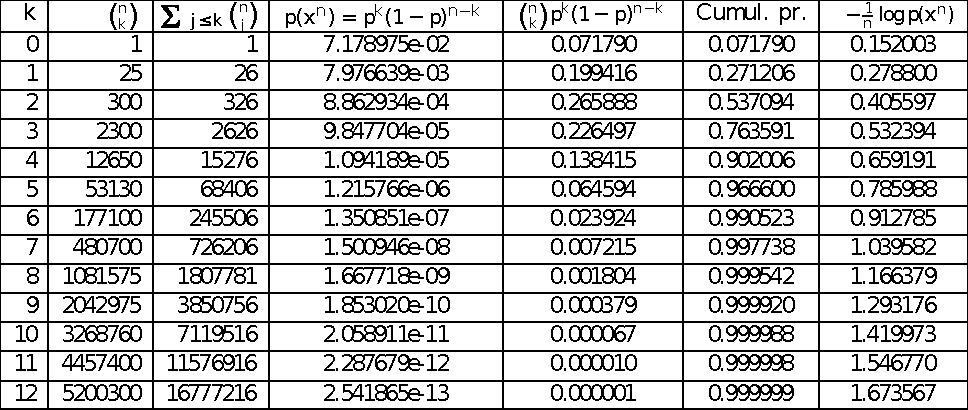
\includegraphics[width=0.8\textwidth]{images/tabex715.pdf}
  \label{fig:tabex715}
  \caption{As sequências com mais de 12 uns foram omitidas pois a probabilidade delas
  é desprezível (e não estão no conjunto típico).}
  \end{figure}

  \examplebreak
  Qual é o tamanho do conjunto $A_{\epsilon}^{(n)}(Z)$? 

  \textit{(solução)}

  Escolhendo $\epsilon = 0.2$, o conjunto típico para $Z$ é o conjunto de sequências para as quais
  $-\frac{1}{n} \log p(z^n) \in \left( H(Z) - \epsilon, H(Z) + \epsilon \right) = (0.269,0.669)$.
  Observado a tabela anterior, para $n=25$, podemos verificar que as sequências em $Z$ típicas 
  são aquelas com 1, 2, 3 ou 4 uns ($k=1,2,3,4$).

  A probabilidade total do conjunto $p( A_{\epsilon}^{(n)}(Z)) = 0.902006 - 0.071790 = 0.830216$
  e o tamanho do conjunto é $\vert A_{\epsilon}^{(n)}(Z) \vert = 15276 - 1 = 15275$. 



  \examplebreak
  \begin{enumerate}[e)]
  \item Considere agora a codificação aleatória para o canal, assim como feito na demonstração
  do teorema da codificação. Suponha que são utilizadas $2^{nR}$ palavras 
  $X^n(1), X^n(2), \ldots, X^n(2^{nR})$, escolhidas uniformemente sobre as $2^n$ possíveis
  sequências binárias de comprimento $n$. Uma dessas palavras é escolhida e enviada através
  do canal. O receptor observa a sequência recebida e tenta encontrar a palavra no código
  que é conjuntamente típica com a sequência recebida. Como discutido anteriormente, 
  isto corresponde a encontrar a palavra de código $X^n(i)$ tal que 
  $Y^n - X^n(i) \in A_{\epsilon}^{(n)}(Z)$. Para uma palavra fixa $x^n(i)$, qual é a probabilidade
  de que a sequência recebida $Y^n$ seja tal que $(x^n(i), Y^n)$ seja conjuntamente típico?
  \end{enumerate}

  \examplebreak
  \textit{(solução)}

  A maneira mais simples de calcular a probabilidade é considerar o canal binário simétrico como
  um canal aditivo $Y=X \oplus Z$, onde $Z \sim \text{Bernoulli}(p)$. Então, a probabilidade
  de que para uma dada palavra, $x^n(i)$, a saída $Y^n$ seja conjuntamente típica com ela
  é igual à probabilidade de que a sequência de ruído $Z^n$ seja típica, isto é, esteja em
  $A_{\epsilon}^{(n)}(Z)$. A sequência de ruído é i.i.d. com distribuição $(1-p,p)$,
  e, como calculado anteriormente, a probabilidade de que esta sequência seja típica é
  $\Pr (A_{\epsilon}^{(n)}(Z)) = 0.830216$. Desta forma, a probabilidade de que a sequência
  recebida não seja conjuntamente típica com a palavra transmitida é $0.169784$.


  \examplebreak
  \begin{enumerate}[f)]
  \item Considere agora uma sequência em particular $y^n = 00000 \ldots 0$.
  Assuma que iremos escolher uma sequência $X^n$ aleatória, distribuída uniformemente
  dentre todas as possíveis $2^n$ sequências binárias de comprimento $n$.
  Qual é a probabilidade de que a sequência escolhida seja conjuntamente típica com $y^n$?
  (Dica: esta é a probabilidade de todas as sequências $x^n$ tais que $y^n - x^n \in A_{\epsilon}^{(n)}(Z)$.)
  \end{enumerate}

  \examplebreak
  \textit{(solução)}

  Como todas as sequências $x^n$ são escolhidas com a mesma probabilidade $((1/2)^n)$,
  a probabilidade de que a sequência $x^n$ escolhida seja conjuntamente típica com a 
  sequência recebida $y^n$ é igual ao número de possíveis pares conjuntamente típicos
  $(x^n, y^n)$ vezes $(1/2)^n$. O número de sequências $x^n$ que são conjuntamente 
  típicas com um dado $y^n$ é igual ao número de $z^n$ típicas, onde $z^n = x^n \oplus y^n$.
  Então, a probabilidade de que uma sequência $x^n$ escolhida aleatoriamente seja típica
  com um dado $y^n$ é 
  $\vert A_{\epsilon}^{(n)}(Z) \vert \times \left( \frac{1}{n} \right)^n = 4.552 \times 10^{-4}$.

  \examplebreak
  \begin{enumerate}[g)]
  \item Considere agora um código com $2^9 = 512$ palavras de comprimento 12
  escolhidas aleatoriamente, com distribuição uniforme entre todas as $2^n$ 
  sequencias de comprimento $n=25$. Uma das palavras, digamos aquela 
  correspondente a $i=1$, é escolhida e enviada através do canal. 
  Como calculado no item (e), a sequencia recebida, com alta probabilidade,
  é conjuntamente típica com a palavra enviada. Qual é a probabilidade de que
  uma ou mais das demais palavras (que foram escolhidas ao acaso, independentemente
  da palavra enviada) ser conjuntamente típica com a sequência recebida?
  (Dica: Você poderá utilizar o limite da união, mas você pode também calcular
  esta probabilidade de forma exata, utilizando os resultados do item (f) e 
  a independência das palavras.)
  \end{enumerate}

  \examplebreak
  \textit{(solução)}

  A partir do item (f) sabemos que cada uma das demais palavras é conjuntamente 
  típica com a sequência recebida com probabilidade $4.552 \times 10^{-4}$, e 
  cada uma dessas palavras é independente. A probabilidade de que nenhuma das 
  511 palavras seja conjuntamente típica com a sequência recebida é portanto
  $(1 - 4.552 \times 10^{-4})^{511} = 0.79241$, e a probabilidade de que ao menos
  uma delas seja conjuntamente típica com a sequência recebida é portanto
  $1-0.79241 = 0.20749$. Utilizando o simples limite da união de eventos,
  teremos que a probabilidade de que uma outra palavra seja conjuntamente típica
  com a sequência recebida será de $4.552 \times 10^{-4} \times 511 = 0.23262$.
  O cálculo anterior fornece um resultado mais exato.

  \examplebreak
  \begin{enumerate}[h)]
  \item Dada que uma palavra em particular foi enviada, a probabilidade de erro
  (feita a média sobre a distribuição de probabilidade do canal e sobre a escolha
  aleatória de outras palavras) pode ser escrita como
  \begin{equation}
  \Pr(\text{Erro} | x^n(1) \text{ enviado}) = \sum_{y^n : y^n \text{ causa erro}} 
  p(y^n | x^n(1)) .
  \end{equation}
  \end{enumerate}

  \examplebreak

  Existem dois tipos de erros: o primeiro ocorre se a sequência recebida $y^n$
  não for conjuntamente típica com a palavra transmitida, e o segundo ocorre se 
  houver uma outra palavra conjuntamente típica com a sequência recebida.
  Utilizando os resultados dos itens anteriores, calcule a probabilidade de erro.
  Por simetria do argumento da codificação aleatória, isto não dependerá
  de qual palavra foi enviada.

  \examplebreak
  \textit{(solução)}

  Existem dois eventos de erro, que são condicionalmente independentes, dada
  a sequência recebida. Na parte anterior, mostramos que a probabilidade condicional
  de erro do segundo tipo é $0.20749$, independente da sequência recebida $y^n$.
  A probabilidade de erro do primeiro tipo é $0.1698$, condicionada à palavra
  de entrada. No item (e) calculamos a probabilidade de que 
  $(x^n(i), Y^n) \notin A_{\epsilon}^{(n)}(X,Y)$, mas isto estava condicionado
  a uma sequência de entrada em particular. Agora, pela simetria e uniformidade
  da construção do código aleatório, esta probabilidade não depende de $x^n(i)$,
  sendo assim, a probabilidade de $(X^n, Y^n) \notin A_{\epsilon}^{(n)}(X,Y)$
  também será igual a esta probabilidade, isto é, $0.1698$.

  \examplebreak
  Podemos então utilizar o limite simples da união de eventos para limitar 
  a probabilidade total de erro $\leq 0.1698 + 0.2075 = 0.3773$.
  Então podemos enviar 512 palavras, de comprimento 25, em um canal binário simétrico
  com probabilidade de troca (\emph{crossover}) 0.1, com probabilidade de erro
  menor do que $0.3773$.

  \examplebreak
  Um calculo um pouco mais acurado da probabilidade de erro pode ser feito
  utilizando o fato condicionante sob a sequência recebida, ambos tipos de erro
  são independentes. Utilizando a simetria do processo de construção do código,
  a probabilidade de erro do primeiro tipo condicionada à sequência recebida
  não depende da sequencia recebida, e é portanto $=0.1698$. Portanto, a probabilidade
  de que nenhum dos tipos de erro ocorra é (utilizando a independência) 
  $=(1-0.1698) (1 - 0.2075) = 0.6579$ e assim, a probabilidade de erro é
  $1 - 0.6579 = 0.3421$.

  \examplebreak
  \textit{(observação)}
 
  \begin{itemize}
  \item Iremos reduzir a probabilidade ao considerar um valor de $\epsilon$ menor e 
  comprimentos $n$ maiores. 
  \item A decodificação utilizada não é ótima. A decodificação ótima é a decodificação
  através da máxima verossimilhança.
  \end{itemize}  

 \end{exercise}

\end{frame}



\begin{frame}[allowframebreaks]
  \frametitle{Codificador e Decodificador como parte do Canal}
  \begin{exercise}[Codificador e Decodificador como parte do Canal]
  Considere um canal binário simétrico com probabilidade de \emph{crossover} 0.1.
  Um possível esquema de codificação para este canal com duas palavras de 
  comprimento 3 é codificar a mensagem $a_1$ como $000$ e $a_2$ como $111$.
  Com este esquema de codificação, podemos considerar a combinação do codificador,
  canal e decodificador como formando um novo canal binário simétrico com duas 
  entradas $a_1$ e $a_2$ e duas saídas $a_1$ e $a_2$.

  \examplebreak
  \begin{enumerate}[a)]
  \item Calcule a probabilidade de \emph{crossover} deste canal.
  \end{enumerate}
  \textit{(solução)}

  Neste novo canal não haverá \emph{crossover} quando nenhum dos 3 bits forem trocados
  ou quando apenas um dos 3 bits forem trocados. Iremos calcular então
  $\Pr(\text{crossover}) = 1 - \Pr(\text{não crossover}) = 1 - ( (1-p)(1-p)(1-p) + 3p(1-p)(1-p) ) = 0.028$. Desta forma, a probabilidade de \emph{crossover} neste novo canal
  será $0.028$. 


  \examplebreak
  \begin{enumerate}[b)]
  \item Qual é a capacidade deste canal em bits por transmissão do canal original?
  \end{enumerate}
  \textit{(solução)}

  A capacidade de um canal binário simétrico com probabilidade de \emph{crossover}
  $p$ é dada por $1 - H(p)$. Neste caso, temos $p=0.028$ e assim
  $1 - H(0.028) = 1 - 0.18426 = 0.81574$ bits para cada palavra de 3 bits. Isto 
  corresponde a $0.81574/3 = 0.27191$ bits por transmissão do canal original.
 
  \examplebreak
  \begin{enumerate}[c)]
  \item Qual é a capacidade do canal binário simétrico original com probabilidade
  de \emph{crossover} 0.1?
  \end{enumerate}
  \textit{(solução)}

  A capacidade do canal original seria de $1 - H(0.1) = 0.531$ bits/transmissão.


  \examplebreak
  \begin{enumerate}[d)]
  \item Prove um resultado geral mostrando que para qualquer canal, considerando o
  codificador e decodificador conjuntamente como um novo canal de mensagens para
  mensagens estimadas não irá aumentar a capacidade em bits por transmissão do
  canal original.
  \end{enumerate}

  \examplebreak

  \textit{(solução)}

  \begin{figure}[h!]
  \centering
  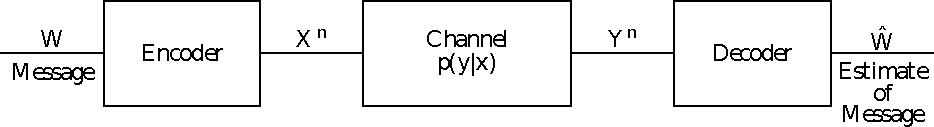
\includegraphics[width=0.8\textwidth]{images/ex716.pdf}
  \label{fig:ex716}
  \end{figure}
 
  Pela desigualdade de processamento de dados temos $I(W;\hat{W}) \leq I(X^n;Y^n)$ e
  assim
  \begin{equation}
  C_W = \max_{p(w)} I(W;\hat{W}) \leq \frac{1}{n} \max_{p(x^n)} I(X^n;Y^n) = C .
  \end{equation}
  Então a capacidade do canal por transmissão não aumentará ao considerar o
  codificador e decodificador como parte do canal.

  \end{exercise}

\end{frame}

